%% abtex2-modelo-trabalho-academico.tex, v-1.9.2 laurocesar
%% Copyright 2012-2014 by abnTeX2 group at http://abntex2.googlecode.com/ 
%%
%% This work may be distributed and/or modified under the
%% conditions of the LaTeX Project Public License, either version 1.3
%% of this license or (at your option) any later version.
%% The latest version of this license is in
%%   http://www.latex-project.org/lppl.txt
%% and version 1.3 or later is part of all distributions of LaTeX
%% version 2005/12/01 or later.
%%
%% This work has the LPPL maintenance status `maintained'.
%% 
%% The Current Maintainer of this work is the abnTeX2 team, led
%% by Lauro César Araujo. Further information are available on 
%% http://abntex2.googlecode.com/
%%
%% This work consists of the files abntex2-modelo-trabalho-academico.tex,
%% abntex2-modelo-include-comandos and abntex2-modelo-references.bib
%%

% ------------------------------------------------------------------------
% ------------------------------------------------------------------------
% abnTeX2: Modelo de Trabalho Academico (tese de doutorado, dissertacao de
% mestrado e trabalhos monograficos em geral) em conformidade com 
% ABNT NBR 14724:2011: Informacao e documentacao - Trabalhos academicos -
% Apresentacao
% ------------------------------------------------------------------------
% ------------------------------------------------------------------------

%-------------------------------------------------------------------------
% Modelo adaptado especificamente para o contexto do PPgSI-EACH-USP por 
% Marcelo Fantinato, com auxílio dos Professores Norton T. Roman, Helton
% H. Bíscaro e Sarajane M. Peres, em 2015, com muitos agradecimentos aos 
% criadores da classe e do modelo base.
%
% 20/06/2017: inclusão de "lista de quadros" com base no especificado em:
% https://github.com/abntex/abntex2/wiki/HowToCriarNovoAmbienteListing,
% de autoria de "Eduardo de Santana Medeiros Alexandre".
%
%-------------------------------------------------------------------------

\documentclass[
	% -- opções da classe memoir --
	12pt,				% tamanho da fonte
	% openright,			% capítulos começam em pág ímpar (insere página vazia caso preciso)
	oneside,			% para impressão apenas no anverso (apenas frente). Oposto a twoside
	a4paper,			% tamanho do papel. 
	% -- opções da classe abntex2 --
	%chapter=TITLE,		% títulos de capítulos convertidos em letras maiúsculas
	%section=TITLE,		% títulos de seções convertidos em letras maiúsculas
	%subsection=TITLE,	% títulos de subseções convertidos em letras maiúsculas
	%subsubsection=TITLE,% títulos de subsubseções convertidos em letras maiúsculas
	% -- opções do pacote babel --
	english,			% idioma adicional para hifenização
	%french,				% idioma adicional para hifenização
	%spanish,			% idioma adicional para hifenização
	brazil				% o último idioma é o principal do documento
	]{abntex2ppgsi}

% ---
% Pacotes básicos 
% ---
% \usepackage{lmodern}			% Usa a fonte Latin Modern			
% \usepackage[T1]{fontenc}		% Selecao de codigos de fonte.
\usepackage[utf8]{inputenc}		% Codificacao do documento (conversão automática dos acentos)
\usepackage{lastpage}			% Usado pela Ficha catalográfica
\usepackage{indentfirst}		% Indenta o primeiro parágrafo de cada seção.
\usepackage{color}				% Controle das cores
\usepackage{graphicx}			% Inclusão de gráficos
\usepackage{microtype} 			% para melhorias de justificação
\usepackage{pdfpages}     %para incluir pdf
\usepackage{algorithm}			%para ilustrações do tipo algoritmo
\usepackage{mdwlist}			%para itens com espaço padrão da abnt
\usepackage[noend]{algpseudocode}			%para ilustrações do tipo algoritmo
		
% ---
% Pacotes adicionais, usados apenas no âmbito do Modelo Canônico do abnteX2
% ---
\usepackage{lipsum}				% para geração de dummy text
% ---

% ---
% Pacotes de citações
% ---
\usepackage[brazilian,hyperpageref]{backref}	 % Paginas com as citações na bibl
\usepackage[alf,abnt-etal-list=0,abnt-etal-text=it]{abntex2cite}	% Citações padrão ABNT

% --- 
% CONFIGURAÇÕES DE PACOTES
% --- 

% ---
% Configurações do pacote backref
% Usado sem a opção hyperpageref de backref
\renewcommand{\backrefpagesname}{Citado na(s) página(s):~}
% Texto padrão antes do número das páginas
\renewcommand{\backref}{}
% Define os textos da citação
\renewcommand*{\backrefalt}[4]{
	\ifcase #1 %
		Nenhuma citação no texto.%
	\or
		Citado na página #2.%
	\else
		Citado #1 vezes nas páginas #2.%
	\fi}%
% ---

% ---
% Informações de dados para CAPA e FOLHA DE ROSTO
% ---

%-------------------------------------------------------------------------
% Comentário adicional do PPgSI - Informações sobre o ``instituicao'':
%
% Não mexer. Deixar exatamente como está.
%
%-------------------------------------------------------------------------
\instituicao{
	UNIVERSIDADE DE SÃO PAULO
	\par
	ESCOLA DE ARTES, CIÊNCIAS E HUMANIDADES
	\par
	PROGRAMA DE PÓS-GRADUAÇÃO EM SISTEMAS DE INFORMAÇÃO}

%-------------------------------------------------------------------------
% Comentário adicional do PPgSI - Informações sobre o ``título'':
%
% Em maiúscula apenas a primeira letra da sentença (do título), exceto 
% nomes próprios, geográficos, institucionais ou Programas ou Projetos ou 
% siglas, os quais podem ter letras em maiúscula também.
%
% O subtítulo do trabalho é opcional.
% Sem ponto final.
%
% Atenção: o título da Dissertação na versão corrigida não pode mudar. 
% Ele deve ser idêntico ao da versão original.
%
%-------------------------------------------------------------------------
\titulo{A Importância da Acessibilidade Digital nas Aplicações Móveis: Um Estudo sobre os Comentários de Usuários no Google Play Store}

%-------------------------------------------------------------------------
% Comentário adicional do PPgSI - Informações sobre o ``autor'':
%
% Todas as letras em maiúsculas.
% Nome completo.
% Sem ponto final.
%-------------------------------------------------------------------------
\autor{\uppercase{Leandro Orlandin}}

%-------------------------------------------------------------------------
% Comentário adicional do PPgSI - Informações sobre o ``local'':
%
% Não incluir o ``estado''.
% Sem ponto final.
%-------------------------------------------------------------------------
\local{São Paulo}

%-------------------------------------------------------------------------
% Comentário adicional do PPgSI - Informações sobre a ``data'':
%
% Colocar o ano do depósito (ou seja, o ano da entrega) da respectiva 
% versão, seja ela a versão original (para a defesa) seja ela a versão 
% corrigida (depois da aprovação na defesa). 
%
% Atenção: Se a versão original for depositada no final do ano e a versão 
% corrigida for entregue no ano seguinte, o ano precisa ser atualizado no 
% caso da versão corrigida. 
% Cuidado, pois o ano da ``capa externa'' também precisa ser atualizado 
% nesse caso.
%
% Não incluir o dia, nem o mês.
% Sem ponto final.
%-------------------------------------------------------------------------
\data{2020}

%-------------------------------------------------------------------------
% Comentário adicional do PPgSI - Informações sobre o ``Orientador'':
%
% Se for uma professora, trocar por ``Profa. Dra.''
% Nome completo.
% Sem ponto final.
%-------------------------------------------------------------------------
\orientador{Prof. Dr. Orientador: Marcelo Medeiros Eler}

%-------------------------------------------------------------------------
% Comentário adicional do PPgSI - Informações sobre o ``Coorientador'':
%
% Opcional. Incluir apenas se houver co-orientador formal, de acordo com o 
% Regulamento do Programa.
%
% Se for uma professora, trocar por ``Profa. Dra.''
% Nome completo.
% Sem ponto final.
%-------------------------------------------------------------------------

%LORLANDIN - RETIRADO O COORIENTADOR
%\coorientador{Prof. Dr. Fulano de Tal}

\tipotrabalho{Dissertação (Mestrado)}

\preambulo{
%-------------------------------------------------------------------------
% Comentário adicional do PPgSI - Informações sobre o texto ``Versão 
% original'':
%
% Não usar para Qualificação.
% Não usar para versão corrigida de Dissertação.
%
%-------------------------------------------------------------------------
%LORLANDIN - RETIRADO POR SER QUALIFICAÇÃO
%Versão original \newline \newline \newline 
%-------------------------------------------------------------------------
% Comentário adicional do PPgSI - Informações sobre o ``texto principal do
% preambulo'':
%
% Para Qualificação, trocar por: Projeto de pesquisa para exame de qualificação apresentado à Escola de Artes, Ciências e Humanidades da Universidade de São Paulo como parte dos requisitos para obtenção do título de Mestre em Ciências pelo Programa de Pós-graduação em Sistemas de Informação.
%
%-------------------------------------------------------------------------
%LORLANDIN - SUBSTITUÍDO CONFORME ORIENTAÇÃO ACIMA - QUALIFICAÇÃO
Projeto de pesquisa para exame de qualificação apresentado à Escola de Artes, Ciências e Humanidades da Universidade de São Paulo como parte dos requisitos para obtenção do título de Mestre em Ciências pelo Programa de Pós-graduação em Sistemas de Informação.
%Dissertação apresentada à Escola de Artes, Ciências e Humanidades da Universidade de São Paulo para obtenção do título de Mestre em Ciências pelo Programa de Pós-graduação em Sistemas de Informação. 
%
\newline \newline Área de concentração: Metodologia e Técnicas da Computação
%-------------------------------------------------------------------------
% Comentário adicional do PPgSI - Informações sobre o texto da ``Versão 
% corrigida'':
%
% Não usar para Qualificação.
% Não usar para versão original de Dissertação.
% 
% Substituir ``xx de xxxxxxxxxxxxxxx de xxxx'' pela ``data da defesa''.
%
%-------------------------------------------------------------------------
%LORLANDIN - RETIRADO POR SER QUALIFICAÇÃO
%\newline \newline \newline Versão corrigida contendo as alterações solicitadas pela comissão julgadora em xx de xxxxxxxxxxxxxxx de xxxx. A versão original encontra-se em acervo reservado na Biblioteca da EACH-USP e na Biblioteca Digital de Teses e Dissertações da USP (BDTD), de acordo com a Resolução CoPGr 6018, de 13 de outubro de 2011.}
% ---
}

% ---
% Configurações de aparência do PDF final

% alterando o aspecto da cor azul
\definecolor{blue}{RGB}{41,5,195}

% informações do PDF
\makeatletter
\hypersetup{
     	%pagebackref=true,
		pdftitle={\@title}, 
		pdfauthor={\@author},
    	pdfsubject={\imprimirpreambulo},
	    pdfcreator={LaTeX com abnTeX2 adaptado para o PPgSI-EACH-USP},
		pdfkeywords={abnt}{latex}{abntex}{abntex2}{qualificação de mestrado}{dissertação de mestrado}{ppgsi}, 
		colorlinks=true,       		% false: boxed links; true: colored links
    	linkcolor=black,          	% color of internal links
    	citecolor=black,        		% color of links to bibliography
    	filecolor=black,      		% color of file links
		urlcolor=black,
		bookmarksdepth=4
}
\makeatother
% --- 

% --- 
% Espaçamentos entre linhas e parágrafos 
% --- 

% O tamanho do parágrafo é dado por:
\setlength{\parindent}{1.25cm}

% Controle do espaçamento entre um parágrafo e outro:
\setlength{\parskip}{0cm}  % tente também \onelineskip
\renewcommand{\baselinestretch}{1.5}

% ---
% compila o indice
% ---
\makeindex
% ---

	% Controlar linhas orfas e viuvas
  \clubpenalty10000
  \widowpenalty10000
  \displaywidowpenalty10000

% ----
% Início do documento
% ----
\begin{document}

% Retira espaço extra obsoleto entre as frases.
\frenchspacing 

% ----------------------------------------------------------
% ELEMENTOS PRÉ-TEXTUAIS
% ----------------------------------------------------------
% \pretextual

% ---
% Capa
% ---
%-------------------------------------------------------------------------
% Comentário adicional do PPgSI - Informações sobre a ``capa'':
%
% Esta é a ``capa'' principal/oficial do trabalho, a ser impressa apenas 
% para os casos de encadernação simples (ou seja, em ``espiral'' com 
% plástico na frente).
% 
% Não imprimir esta ``capa'' quando houver ``capa dura'' ou ``capa brochura'' 
% em que estas mesmas informações já estão presentes nela.
%
%-------------------------------------------------------------------------
\imprimircapa
% ---

% ---
% Folha de rosto
% (o * indica que haverá a ficha bibliográfica)
% ---
\imprimirfolhaderosto*
% ---

% ---
% Inserir a autorização para reprodução e ficha bibliografica
% ---

%-------------------------------------------------------------------------
% Comentário adicional do PPgSI - Informações sobre o texto da 
% ``autorização para reprodução e ficha bibliografica'':
%
% Página a ser usada apenas para Dissertação (tanto na versão original 
% quanto na versão corrigida).
%
% Solicitar a ficha catalográfica na Biblioteca da EACH. 
% Duas versões devem ser solicitadas, em dois momentos distintos: uma vez 
% para a versão original, e depois outra atualizada para a versão 
% corrigida.
%
% Atenção: esta página de ``autorização para reprodução e ficha 
% catalográfica'' deve ser impressa obrigatoriamente no verso da folha de 
% rosto.
%
% Não usar esta página para Qualificação.
%
% Substitua o arquivo ``fig_ficha_catalografica.pdf'' abaixo referenciado 
% pelo PDF elaborado pela Biblioteca
%
%-------------------------------------------------------------------------
%LORLANDIN - RETIRADO POR SER QUALIFICAÇÃO
%\begin{fichacatalografica}
%    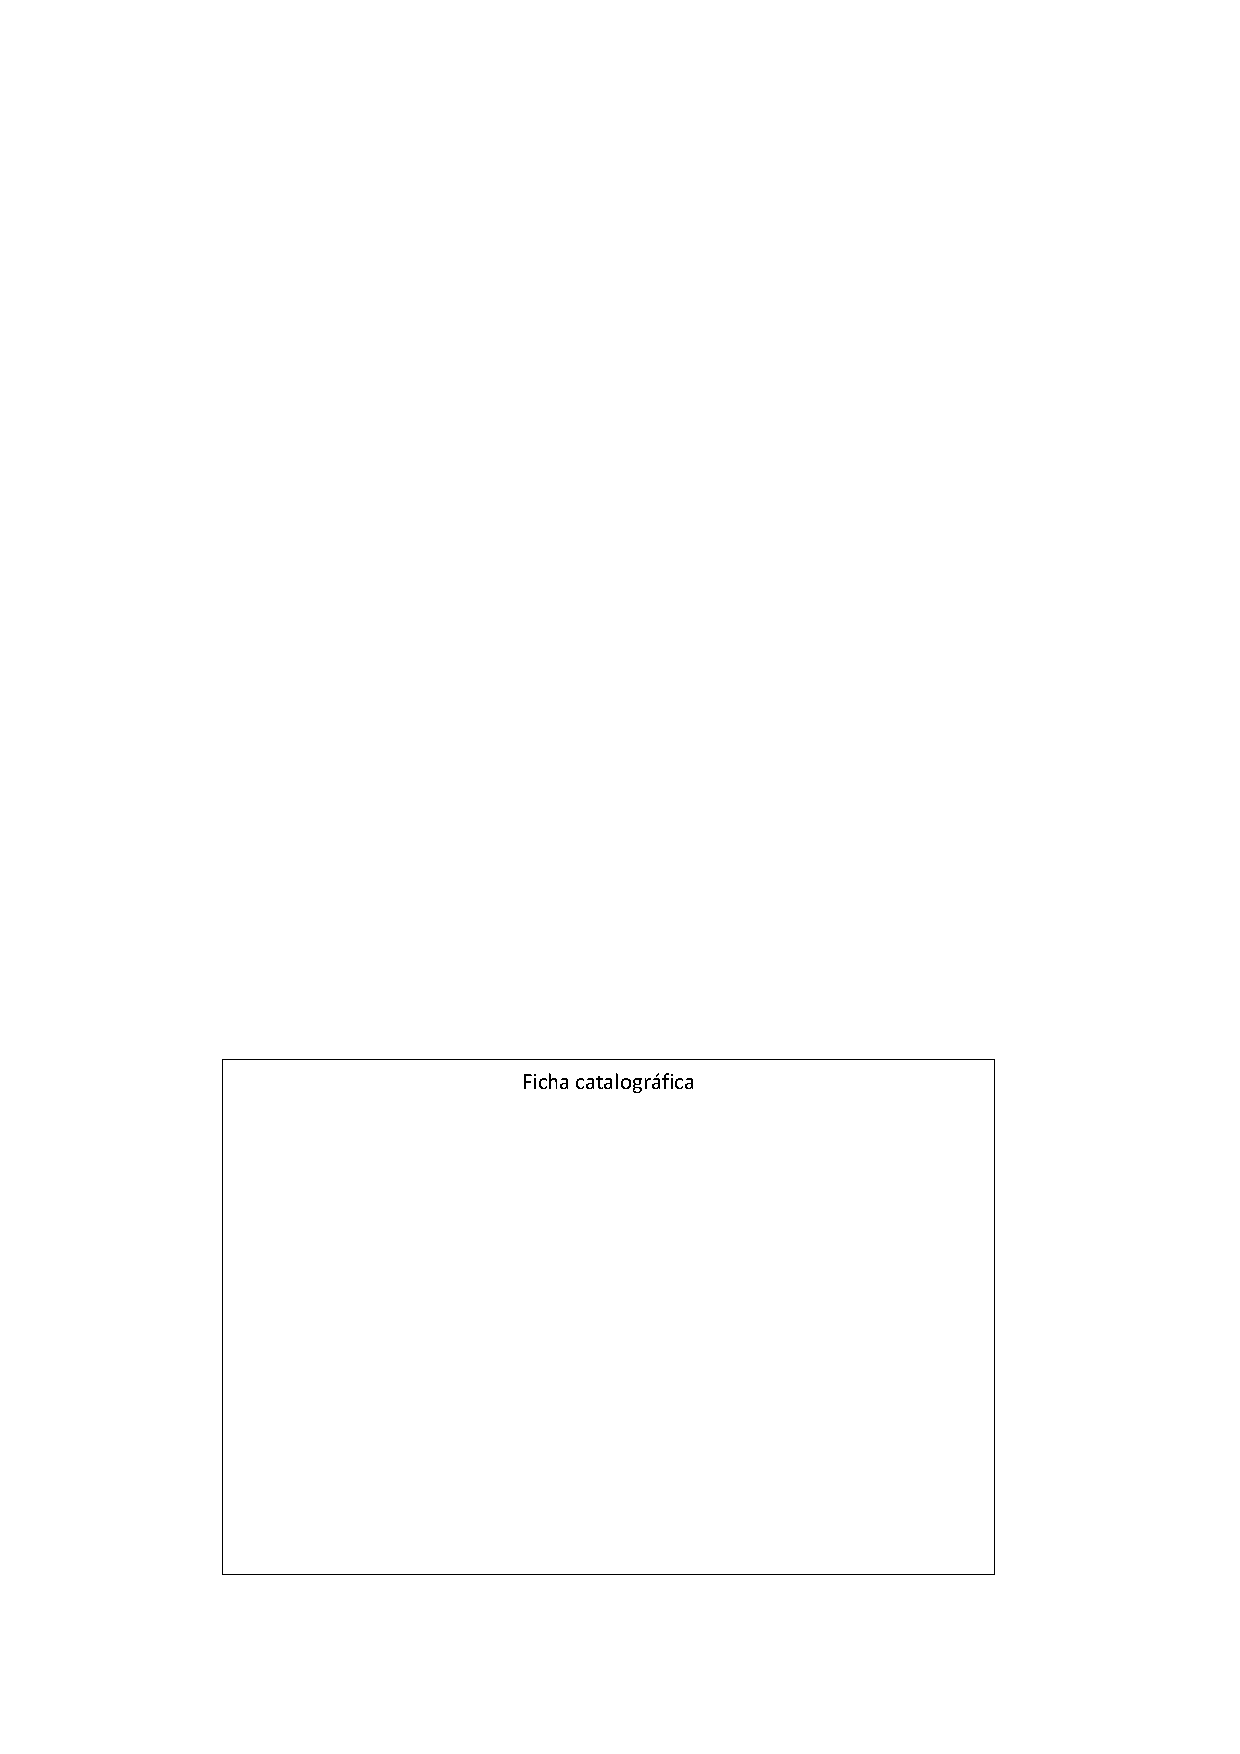
\includepdf{fig_ficha_catalografica.pdf}
%\end{fichacatalografica}



% ---
% Inserir errata
% ---
%-------------------------------------------------------------------------
% Comentário adicional do PPgSI - Informações sobre ``Errata'':
%
% Usar esta página de errata apenas em casos de excepcionais, e apenas 
% para a versão corrigida da Dissertação. Por exemplo, quando depois de
% já depositada e publicada a versão corrigida, ainda assim verifica-se
% a necessidade de alguma correção adicional.
%
% Se precisar usar esta página, busque a forma correta (o modelo correto) 
% para fazê-lo, de acordo com a norma ABNT.
%
% Não usar esta página para versão original de Dissertação.
% Não usar esta página para Qualificação.
%
%-------------------------------------------------------------------------
%LORLANDIN - RETIRADO POR SER QUALIFICAÇÃO
%\begin{errata}
%Elemento opcional para versão corrigida, depois de depositada.
%\end{errata}
% ---

% ---
% Inserir folha de aprovação
% ---

\begin{folhadeaprovacao}

%-------------------------------------------------------------------------
% Comentário adicional do PPgSI - Informações sobre ``Folha da aprovação'':
%
% Página a ser usada apenas para Dissertação.
%
% Não usar esta página para Qualificação.
%
% Substituir ``Fulano de Tal'' pelo nome completo do autor do trabalho, com 
% apenas as iniciais em maiúsculo.
%
% Substituir ``___ de ______________ de ______'' por: 
%     - Para versão original de Dissertação: deixar em branco, pois a data 
%       pode mudar, mesmo que ela já esteja prevista.
%     - Para versão corrigida de Dissertação: usar a data em que a defesa 
%       efetivamente ocorreu.
%
%-------------------------------------------------------------------------

%LORLANDIN - RETIRADO POR SER QUALIFICAÇÃO
%\noindent Dissertação de autoria de Fulano de Tal, sob o título \textbf{``\imprimirtitulo''}, apresentada à Escola de Artes, Ciências e Humanidades da Universidade de São Paulo, para obtenção do título de Mestre em Ciências pelo Programa de Pós-graduação em Sistemas de Informação, na área de concentração Metodologia e Técnicas da Computação, aprovada em \_\_\_\_\_\_\_ de \_\_\_\_\_\_\_\_\_\_\_\_\_\_\_\_\_\_\_\_\_\_ de \_\_\_\_\_\_\_\_\_\_ pela comissão julgadora constituída pelos doutores:

\vspace*{3cm}

\begin{center}
%-------------------------------------------------------------------------
% Comentário adicional do PPgSI - Informações sobre ``assinaturas'':
%
% Para versão original de Dissertação: deixar em 
% branco (ou seja, assim como está abaixo), pois os membros da banca podem
% mudar, mesmo que eles já estejam previstos.
% 
% Para versão corrigida de Dissertação: usar os dados dos examinadores que 
% efetivamente participaram da defesa. 
% 
% Para versão corrigida de Dissertação: em caso de ``professora'', trocar 
% por ``Profa. Dra.'' 
% 
% Para versão corrigida de Dissertação: ao colocar os nomes dos 
% examinadores, remover o sublinhado
% 
% Para versão corrigida de Dissertação: ao colocar os nomes dos 
% examinadores, usar seus nomes completos, exatamente conforme constam em 
% seus Currículos Lattes
% 
% Para versão corrigida de Dissertação: ao colocar os nomes das 
% instituições, remover o sublinhado e remover a palavra ``Instituição:''
%
% Para a versão corrigida de Dissertação: remova o texto “Instituição: ”, 
% ou seja, coloque apenas/diretamente o nome da instituição.
%
% Não abreviar os nomes das instituições.
%
%-------------------------------------------------------------------------
\_\_\_\_\_\_\_\_\_\_\_\_\_\_\_\_\_\_\_\_\_\_\_\_\_\_\_\_\_\_\_\_\_\_\_\_\_\_\_\_\_\_\_\_\_\_\_\_\_\_\_\_\_\_\_\_
\vspace*{0.2cm} 
\\ \textbf{Prof. Dr. \_\_\_\_\_\_\_\_\_\_\_\_\_\_\_\_\_\_\_\_\_\_\_\_\_\_\_\_\_\_\_\_\_\_\_\_\_\_\_\_\_\_\_\_\_\_\_\_\_\_\_\_\_\_\_\_\_\_\_\_\_\_} 
\\ \vspace*{0.2cm} 
Instituição: \_\_\_\_\_\_\_\_\_\_\_\_\_\_\_\_\_\_\_\_\_\_\_\_\_\_\_\_\_\_\_\_\_\_\_\_\_\_\_\_\_\_\_\_\_\_\_\_\_\_\_\_\_\_\_\_\_\_ 
\\ \vspace*{0.2cm}
Presidente 

\vspace*{2cm}

\_\_\_\_\_\_\_\_\_\_\_\_\_\_\_\_\_\_\_\_\_\_\_\_\_\_\_\_\_\_\_\_\_\_\_\_\_\_\_\_\_\_\_\_\_\_\_\_\_\_\_\_\_\_\_\_
\vspace*{0.2cm} 
\\ \textbf{Prof. Dr. \_\_\_\_\_\_\_\_\_\_\_\_\_\_\_\_\_\_\_\_\_\_\_\_\_\_\_\_\_\_\_\_\_\_\_\_\_\_\_\_\_\_\_\_\_\_\_\_\_\_\_\_\_\_\_\_\_\_\_\_\_\_} 
\\ \vspace*{0.2cm} 
Instituição: \_\_\_\_\_\_\_\_\_\_\_\_\_\_\_\_\_\_\_\_\_\_\_\_\_\_\_\_\_\_\_\_\_\_\_\_\_\_\_\_\_\_\_\_\_\_\_\_\_\_\_\_\_\_\_\_\_\_

\vspace*{2cm}

\_\_\_\_\_\_\_\_\_\_\_\_\_\_\_\_\_\_\_\_\_\_\_\_\_\_\_\_\_\_\_\_\_\_\_\_\_\_\_\_\_\_\_\_\_\_\_\_\_\_\_\_\_\_\_\_
\vspace*{0.2cm} 
\\ \textbf{Prof. Dr. \_\_\_\_\_\_\_\_\_\_\_\_\_\_\_\_\_\_\_\_\_\_\_\_\_\_\_\_\_\_\_\_\_\_\_\_\_\_\_\_\_\_\_\_\_\_\_\_\_\_\_\_\_\_\_\_\_\_\_\_\_\_} 
\\ \vspace*{0.2cm} 
Instituição: \_\_\_\_\_\_\_\_\_\_\_\_\_\_\_\_\_\_\_\_\_\_\_\_\_\_\_\_\_\_\_\_\_\_\_\_\_\_\_\_\_\_\_\_\_\_\_\_\_\_\_\_\_\_\_\_\_\_

\vspace*{2cm}

\_\_\_\_\_\_\_\_\_\_\_\_\_\_\_\_\_\_\_\_\_\_\_\_\_\_\_\_\_\_\_\_\_\_\_\_\_\_\_\_\_\_\_\_\_\_\_\_\_\_\_\_\_\_\_\_
\vspace*{0.2cm} 
\\ \textbf{Prof. Dr. \_\_\_\_\_\_\_\_\_\_\_\_\_\_\_\_\_\_\_\_\_\_\_\_\_\_\_\_\_\_\_\_\_\_\_\_\_\_\_\_\_\_\_\_\_\_\_\_\_\_\_\_\_\_\_\_\_\_\_\_\_\_} 
\\ \vspace*{0.2cm} 
Instituição: \_\_\_\_\_\_\_\_\_\_\_\_\_\_\_\_\_\_\_\_\_\_\_\_\_\_\_\_\_\_\_\_\_\_\_\_\_\_\_\_\_\_\_\_\_\_\_\_\_\_\_\_\_\_\_\_\_\_

\end{center}

\end{folhadeaprovacao}
% ---

% ---
% Dedicatória
% ---
%-------------------------------------------------------------------------
% Comentário adicional do PPgSI - Informações sobre ``Dedicatória'': 
%
% Opcional para Dissertação.
% Não sugerido para Qualificação.
% 
%-------------------------------------------------------------------------

%LORLANDIN - RETIRADO POR SER QUALIFICAÇÃO - REINSERIR PARA A DISSERTAÇÃO
%\begin{dedicatoria}
%   \vspace*{\fill}
%   \centering
%   \noindent
%   \textit{Escreva aqui sua dedicatória, se desejar, ou remova esta página...} 
%	 \vspace*{\fill}
%\end{dedicatoria}
% ---

% ---
% Agradecimentos
% ---
%-------------------------------------------------------------------------
% Comentário adicional do PPgSI - Informações sobre ``Agradecimentos'': 
%
% Opcional para Dissertação.
% Não sugerido para Qualificação.
% 
% 
% Financiamentos recebidos durante o projeto de mestrado, vindos de qualquer 
% agência de fomento, devem ser mencionados na seção de agradecimentos da dissertação. 
% Isso se aplica não apenas a bolsas de estudo, mas a qualquer tipo de financiamento, 
% tais como para apoio a participação em eventos, compra de materiais, traduções etc. 
% Especificamente para financiamento da Capes, siga as instruções contidas na portaria 
% 206, de 4/set/2018; para outras agências de fomento, procure as regras apropriadas.
%
% Portaria Capes 206, de 4/set/2018: 
% http://ppgsi.each.usp.br/arquivos/Portaria_0783227_Portaria_CAPES_DOU___206_de_2018.pdf 
%
%
%-------------------------------------------------------------------------

%LORLANDIN - RETIRADO POR SER QUALIFICAÇÃO
%\begin{agradecimentos}
%Texto de exemplo, texto de exemplo, texto de exemplo, texto de exemplo, texto de exemplo, texto de exemplo, texto de exemplo, texto de exemplo, texto de exemplo, texto de exemplo, texto de exemplo, texto de exemplo, texto de exemplo, texto de exemplo, texto de exemplo, texto de exemplo, texto de exemplo, texto de exemplo, texto de exemplo, texto de exemplo, texto de exemplo, texto de exemplo.

%Texto de exemplo, texto de exemplo, texto de exemplo, texto de exemplo, texto de exemplo, texto de exemplo, texto de exemplo, texto de exemplo, texto de exemplo, texto de exemplo, texto de exemplo, texto de exemplo, texto de exemplo, texto de exemplo, texto de exemplo, texto de exemplo, texto de exemplo, texto de exemplo, texto de exemplo, texto de exemplo, texto de exemplo, texto de exemplo.

%Texto de exemplo, texto de exemplo, texto de exemplo, texto de exemplo, texto de exemplo, texto de exemplo, texto de exemplo, texto de exemplo, texto de exemplo, texto de exemplo, texto de exemplo, texto de exemplo, texto de exemplo, texto de exemplo, texto de exemplo, texto de exemplo, texto de exemplo, texto de exemplo, texto de exemplo, texto de exemplo, texto de exemplo, texto de exemplo.

%Texto de exemplo, texto de exemplo, texto de exemplo, texto de exemplo, texto de exemplo, texto de exemplo, texto de exemplo, texto de exemplo, texto de exemplo, texto de exemplo, texto de exemplo, texto de exemplo, texto de exemplo, texto de exemplo, texto de exemplo, texto de exemplo, texto de exemplo, texto de exemplo, texto de exemplo, texto de exemplo, texto de exemplo, texto de exemplo.

%Texto de exemplo, texto de exemplo, texto de exemplo, texto de exemplo, texto de exemplo, texto de exemplo, texto de exemplo, texto de exemplo, texto de exemplo, texto de exemplo, texto de exemplo, texto de exemplo, texto de exemplo, texto de exemplo, texto de exemplo, texto de exemplo, texto de exemplo, texto de exemplo, texto de exemplo, texto de exemplo, texto de exemplo, texto de exemplo.
%\end{agradecimentos}
% ---

% ---
% Epígrafe
% ---
%-------------------------------------------------------------------------
% Comentário adicional do PPgSI - Informações sobre ``Epígrafe'': 
%
% Opcional para Dissertação.
% Não sugerido para Qualificação.
% 
%-------------------------------------------------------------------------
%LORLANDIN - RETIRADO POR SER QUALIFICAÇÃO
%\begin{epigrafe}
%    \vspace*{\fill}
%	\begin{flushright}
%		\textit{``Escreva aqui uma epígrafe, se desejar, ou remova esta página...''\\
%		(Autor da epígrafe)}
%	\end{flushright}
%\end{epigrafe}
% ---

% ---
% RESUMOS
% ---

% resumo em português
\setlength{\absparsep}{18pt} % ajusta o espaçamento dos parágrafos do resumo
%\begin{resumo}

%-------------------------------------------------------------------------
% Comentário adicional do PPgSI - Informações sobre ``referência'':
% 
% Troque os seguintes campos pelos dados de sua Dissertação (mantendo a 
% formatação e pontuação):
%   - SOBRENOME
%   - Nome1
%   - Nome2
%   - Nome3
%   - Título do trabalho: subtítulo do trabalho
%   - AnoDeDefesa
%
% Mantenha todas as demais informações exatamente como estão.
% 
% [Não usar essas informações de ``referência'' para Qualificação]
%
%-------------------------------------------------------------------------
%LORLANDIN - RETIRADO POR SER QUALIFICAÇÃO
%\begin{flushleft}
%SOBRENOME, Nome1 Nome2 Nome3. \textbf{Título do trabalho}: subtítulo do trabalho. \imprimirdata. \pageref{LastPage} f. Dissertação (Mestrado em Ciências) – Escola de Artes, Ciências e Humanidades, Universidade de São Paulo, São Paulo, AnoDeDefesa.
%\end{flushleft}

%Escreva aqui o texto do seu resumo... (redigido em parágrafo único, no máximo em uma página, contendo no ``máximo 500 palavras'', e apresentando um resumo de todos o seu trabalho, incluindo objetivos, metodologia, resultados e conclusões; não inclua apenas a contextualização até chegar nos objetivos, é importante fazer um resumo de todos os capítulos do texto, até chegar à conclusão). Texto de exemplo, texto de exemplo, texto de exemplo, texto de exemplo, texto de exemplo, texto de exemplo, texto de exemplo, texto de exemplo, texto de exemplo, texto de exemplo, texto de exemplo, texto de exemplo, texto de exemplo, texto de exemplo, texto de exemplo, texto de exemplo, texto de exemplo, texto de exemplo, texto de exemplo, texto de exemplo, texto de exemplo, texto de exemplo.

%Palavras-chaves: Palavra1. Palavra2. Palavra3. etc.
%\end{resumo}

% resumo em inglês
%-------------------------------------------------------------------------
% Comentário adicional do PPgSI - Informações sobre ``resumo em inglês''
% 
% Caso a Qualificação ou a Dissertação inteira seja elaborada no idioma inglês, 
% então o ``Abstract'' vem antes do ``Resumo''.
% 
%-------------------------------------------------------------------------
%LORLANDIN - RETIRADO POR SER QUALIFICAÇÃO
%\begin{resumo}[Abstract]
%\begin{otherlanguage*}{english}

%-------------------------------------------------------------------------
% Comentário adicional do PPgSI - Informações sobre ``referência em inglês''
% 
% Troque os seguintes campos pelos dados de sua Dissertação (mantendo a 
% formatação e pontuação):
%     - SURNAME
%     - FirstName1
%     - MiddleName1
%     - MiddleName2
%     - Work title: work subtitle
%     - DefenseYear (Ano de Defesa)
%
% Mantenha todas as demais informações exatamente como estão.
%
% [Não usar essas informações de ``referência'' para Qualificação]
%
%-------------------------------------------------------------------------
%LORLANDIN - RETIRADO POR SER QUALIFICAÇÃO
%\begin{flushleft}
%SURNAME, FirstName MiddleName1 MiddleName2. \textbf{Work title}: work subtitle. \imprimirdata. \pageref{LastPage} p. Dissertation (Master of Science) – School of Arts, Sciences and Humanities, University of São Paulo, São Paulo, DefenseYear. 
%\end{flushleft}

%Write here the English version of your ``Resumo''. Example text, example text, example text, example text, example text, example text, example text, example text, example text, example text, example text, example text, example text, example text, example text, example text, example text, example text, example text, example text, example text, example text, example text, example text, example text, example text, example text, example text, example text, example text, example text, example text, example text, example text, example text, example text, example text, example text, example text, example text, example text, example text, example text, example text, example text, example text, example text.

%LORLANDIN - RETIRADO POR SER QUALIFICAÇÃO
%Keywords: Keyword1. Keyword2. Keyword3. etc.
%\end{otherlanguage*}
%\end{resumo}

% ---
% ---
% inserir lista de figuras
% ---
\pdfbookmark[0]{\listfigurename}{lof}
\listoffigures*
\cleardoublepage
% ---

% ---
% inserir lista de algoritmos
% ---
\pdfbookmark[0]{\listalgorithmname}{loa}
\listofalgorithms
\cleardoublepage

% ---
% inserir lista de quadros
% ---
\pdfbookmark[0]{\listofquadrosname}{loq}
\listofquadros*
\cleardoublepage


% ---
% inserir lista de tabelas
% ---
\pdfbookmark[0]{\listtablename}{lot}
\listoftables*
\cleardoublepage
% ---

% ---
% inserir lista de abreviaturas e siglas
% ---
%-------------------------------------------------------------------------
% Comentário adicional do PPgSI - Informações sobre ``Lista de abreviaturas 
% e siglas'': 
%
% Opcional.
% Uma vez que se deseja usar, é necessário manter padrão e consistência no
% trabalho inteiro.
% Se usar: inserir em ordem alfabética.
%
%-------------------------------------------------------------------------
%LORLANDIN - RETIRADO POR SER QUALIFICAÇÃO
%\begin{siglas}
%  \item[Sigla/abreviatura 1] Definição da sigla ou da abreviatura por extenso
%  \item[Sigla/abreviatura 2] Definição da sigla ou da abreviatura por extenso
%  \item[Sigla/abreviatura 3] Definição da sigla ou da abreviatura por extenso
%  \item[Sigla/abreviatura 4] Definição da sigla ou da abreviatura por extenso
%  \item[Sigla/abreviatura 5] Definição da sigla ou da abreviatura por extenso
%  \item[Sigla/abreviatura 6] Definição da sigla ou da abreviatura por extenso
%  \item[Sigla/abreviatura 7] Definição da sigla ou da abreviatura por extenso
%  \item[Sigla/abreviatura 8] Definição da sigla ou da abreviatura por extenso
%  \item[Sigla/abreviatura 9] Definição da sigla ou da abreviatura por extenso
%  \item[Sigla/abreviatura 10] Definição da sigla ou da abreviatura por extenso
%\end{siglas}
% ---

% ---
% inserir lista de símbolos
% ---
%-------------------------------------------------------------------------
% Comentário adicional do PPgSI - Informações sobre ``Lista de símbolos'': 
%
% Opcional.
% Uma vez que se deseja usar, é necessário manter padrão e consistência no
% trabalho inteiro.
% Se usar: inserir na ordem em que aparece no texto.
% 
%-------------------------------------------------------------------------
\begin{simbolos}
  \item[$ \Gamma $] Letra grega Gama
  \item[$ \Lambda $] Lambda
  \item[$ \zeta $] Letra grega minúscula zeta
  \item[$ \in $] Pertence
\end{simbolos}
% ---

% ---
% inserir o sumario
% ---
\pdfbookmark[0]{\contentsname}{toc}
\tableofcontents*
\cleardoublepage
% ---



% ----------------------------------------------------------
% ELEMENTOS TEXTUAIS
% ----------------------------------------------------------
\textual



%-------------------------------------------------------------------------
% Comentário adicional do PPgSI - Informações sobre ``títulos de seções''
% 
% Para todos os títulos (seções, subseções, tabelas, ilustrações, etc.):
%
% Em maiúscula apenas a primeira letra da sentença (do título), exceto 
% nomes próprios, geográficos, institucionais ou Programas ou Projetos ou
% siglas, os quais podem ter letras em maiúscula também.
%
%-------------------------------------------------------------------------
\chapter{Introdução}


\section{Contextualização}

Importante parcela da população mundial possui algum tipo de deficiência que impossibilita a execução das mais diversas atividades cotidianas. De acordo com a Organização Mundial da Saúde - OMS (\textit{World Health Organization - WHO}) \footnote{http://documents.worldbank.org/curated/en/665131468331271288/Main-report} as estimativas são de que este público seja superior a 1 bilhão de pessoas. Considerando a população brasileira, as estimativas do censo de 2010\footnote{https://biblioteca.ibge.gov.br/visualizacao/periodicos/94/cd\_2010\_religiao\_deficiencia.pdf} são de que aproximadamente 18,8\% apresenta algum tipo de deficiência visual, 5,1\% deficiência auditiva, 7\% deficiência motora e 1,4\% deficiência mental ou intelectual. Importante salientar também que estes percentuais se agravam para população com idade a partir de 65 anos.

Paralelo a este cenário, identifica-se também um aumento considerável do número de softwares para dispositivos móveis\footnote{https://www.statista.com/statistics/266210/number-of-available-applications-in-the-google-play-store/} denominados como aplicações móveis (ou apenas \textit{apps}). Esta explosão de \textit{apps} disponíveis para serem instalados e utilizados em celulares, tablets ou até mesmo em computadores, passou de 30 mil em 2009 para mais de 3 milhões em 2018, evidenciando assim a importância dos mesmos em muitos aspectos de nossas atividades cotidianas \cite{storeanalysis}.

A partir dos fatores acima, índices de deficiência da população e utilização dos dispositivos móveis no cotidiano, atesta-se a importância da acessibilidade digital neste novo panorama mundial, essa representando a capacidade do software de ser utilizado independentemente da condição física, mental ou intelectual do usuário \cite{w3cwai}. Como formas de intensificar o uso de aplicações acessíveis, em muitos países, a acessibilidade digital trata-se de uma obrigação legal \cite{Silva2018survey}. 

Com a intenção de endereçar este tema auxiliando os designers e desenvolvedores de software a criar produtos acessíveis, vários padrões têm sido propostos e amplamente utilizados, principalmente aqueles ligados ao \textit{World Wide Web Consortium - W3C} \cite{wcag} e ao \textit{BBC Guidelines} \cite{bbc}. No âmbito nacional destaca-se o Modelo de Acessibilidade em Governo Eletrônico, ou simplesmente eMAG \cite{emag}. Todavia, é possível observar em estudos que ainda existe uma falta de acessibilidade nas aplicações \cite{smartcities,Eler2018mate,Quispe2018accessibility,Serra2015accessibility,Yan2019currentstatus}.

É fundamental que não apenas os requisitos funcionais sejam garantidos pelas aplicações, mas também a disponibilização das mesmas considerando sua acessibilidade \cite{Oliveira2017strategies}. No âmbito de \textit{apps}, tem-se como importante característica suas constantes atualizações através de novas versões nas lojas de aplicativos (e.g. Google Play Store) \cite{nayebi,Palompa2018crowdsourcing}. Este processo de frequente revisão ao longo do tempo torna as aplicações mais maduras, com inclusão de novas funcionalidades e correções de erros.

Em muitos estudos identifica-se que tanto as classificações quanto os comentários dos usuários nas lojas de aplicativos são um importante direcionador para os desenvolvedores no momento do lançamento de novas versões \cite{Ciurumelea2017analyzing,Li2018MobileAE,Ortega2015thesis,Palomba2015userreviews,Palompa2018crowdsourcing,Pelloni2018becloma}. Considerando assim que os comentários orientam o desenvolvimento das \textit{apps} e que mesmo as mais maduras e populares apresentam problemas de acessibilidade \cite{Eler2018mate}, a dúvida que surge é se os usuários reportam suas dificuldades referentes à acessibilidade nas lojas de aplicativos.



\section{Problema de Pesquisa}

Diferentes taxonomias são empregadas nos estudos dos comentários \cite{Ciurumelea2017analyzing,Sorbo2017surf,Iacob2013retrieving,Iacob2014online,Li2018MobileAE,Mcilroy2016analyzing,Ortega2015thesis,Pagano2013userfeedback,Panichella2015how,Pelloni2018becloma}, e apesar de alguns destes trabalhos citarem inclusive interfaces com usuário, não se observa estudos que possuam detalhamento a respeito dos problemas relacionados à acessibilidade digital.

Desta forma, esta proposta de pesquisa visa realizar um estudo amplo e generalizado sobre os comentários dos usuários envolvendo o tema acessibilidade na loja de aplicativos móveis \textit{Google Play Store}.

As justificativas que visam embasar esta investigação pretendem 
i) identificar se existe um volume significativo de comentários envolvendo acessibilidade e sua distribuição de acordo com as categorias dos \textit{apps},
ii) analisar a diversificação dos comentários de acordo com padrões internacionais de acessibilidade \cite{bbc} e
ii) por fim se existe um relacionamento entre a classificação do comentário de acordo com a acessibilidade e à respectiva nota dada ao aplicativo pelo próprio usuário.

Com este estudo, será possível confirmar a existência de uma pressão dos usuários frente aos desenvolvedores e empresas de aplicativos no que diz respeito às funcionalidades envolvendo acessibilidade.


\section{Metodologia}

%falar bem rapidamente como chegaremos lá
%selecionaremos um conjunto de aplicações
%implementar ferramentas para coletar estes comentários
%analisaremos estes comentários
%definiremos palavras chave
%validação manual
%utilizaremos PLN (mas precisamos definir para quê utilizar a mesma) se dividirmos quantos tópicos a pessoa fala em cada comentários seria interessante
%quando a pessoa apenas reclama de algo a nota é ruim, porém quando existem outros assuntos envolvidos e algum deles pode ser elogios, a nota pode ser melhor.....
%análise de sentimento para extrair algo

Será definido um conjunto de aplicações móveis, com a condição inicial de que possuam versões de suas instalações (arquivos de instalação com extensão \textit{apk}) disponíveis no repositório F-Droid\footnote{https://f-droid.org/}. Este requisito permitirá que a pesquisa seja posteriormente evoluída, através de comparações entre os problemas de acessibilidade encontrados em diferentes versões do software, fora do escopo deste projeto. É importante que o levantamento selecione aplicações de diferentes categorias, como por exemplo: navegação, finanças e leitura.

Uma nova ferramenta, em linguagem Python, será implementada para coletar os comentários dos aplicativos e validar a existência de versões do softaware de instalação no repositório de F-Droid. Esta condição inicial de validação poderá ser excluída se por ventura o conjunto for restrito a determinadas categorias ou mesmo possuam reduzido número de comentários envolvendo acessibilidade.

Com base no \textit{W3C} \cite{wcag} e no \textit{BBC Guidelines} \cite{bbc}, serão estabelecidas palavras-chave que, em existindo no comentário, indicarão a possibilidade do mesmo se referir a uma diretriz de acessibilidade.

Em posse dos comentários e das palavras-chave, será possível iniciar um processo de averiguação manual se os mesmos abordam o tema acessibilidade e qual foi a mensagem transmitida pelo usuário (pedido de correção ou cumprimentos pelo aplicativo). Esta averiguação, poderá ser feita em parceria com outro projeto que envolva Processamento de Linguagem Natural (PLN).

Como forma de complementar a verificação utilizando-se de PLN, poderá ser utilizado um processo de Análise de Sentimento (AS), conforme abordado em literatura como uma forma de melhorar o processo investigativo\cite{Panichella2015how}.
%#comentário# ESTA PARTE DE PLN E AS PRECISAM SER MELHOR EXPLICADAS


\section{Organização}
%O que teremos em qual capítulo
%Dar um panorama geral do documento
* * * * * * * * * * * * * * * * * * * * * * 

* * * * * * \underline{A ELABORAR AINDA} * * * * * * *

* * * * * * * * * * * * * * * * * * * * * * 


\chapter{Revisão de Literatura}

Segundo o site \textit{Dicio - Dicionário Online de Português}, a definição de acessibilidade pode ser dada como sendo \textit{a propriedade de material confeccionado para que qualquer pessoa tenha acesso, consiga ver, usar, compreender, principalmente de material que se destina à inclusão social de pessoas com alguma deficiência} \footnote{https://www.dicio.com.br/acessibilidade/}. Trata-se da possibilidade e condição de qualquer indivíduo alcançar os elementos funcionais do ambiente construído, para assim permitir sua utilização \cite{camilamaster}.

Para o caso de acessibilidade digital, e conforme visto anteriormente, a mesma representa a capacidade de um software ser utilizado, independentemente da condição física, mental ou intelectual do usuário \cite{w3cwai}. Trata-se da flexibilidade do software em se adaptar às necessidades de cada usuário, suas preferências e limitações \cite{camilamaster}. Este fator torna-se mais importante no contexto mundial atual em decorrência dos índices de pessoas com algum tipo de deficiência e da alta demanda por \textit{apps} em dispositivos móveis \cite{storeanalysis}.

Normalmente a acessibilidade digital é associada exclusivamente às dificuldades motoras, físicas ou sensoriais dos indivíduos com necessidades especiais, sendo desconsiderada importante parcela da população, como por exemplo idosos ou crianças. Uma aplicação que não seja acessível a um indivíduo não pode ser considerada eficaz, eficiente ou agradável ao mesmo \cite{santarosa}.

\section{Padrões de Acessibilidade}
Para atender a estas necessidades, diversos padrões foram definidos, com destaque para o WCAG, BBC Guidelines e eMAG, utilizados nesta proposta de pesquisa. Esta carência foi fortemente identificada no decorrer da década de 1990, quando se ampliou a utilização da internet pela sociedade. Destacam-se como principais promotores dois consórcios internacionais: o W3C (Consórcio para a Web) e a WAI (Iniciativa para a Acessibilidade na Rede), responsáveis pelo estabelecimento de padrões e protocolos que sistemas computacionais deveriam seguir para serem considerados acessíveis \cite{passerino}.

\subsection{WCAG}
O \textit{Web Content Accessibility Guidelines}, ou WCAG2.0 \footnote{https://www.w3.org/WAI/intro/wcag}, trata-se de um documento elaborado pela W3C, com conteúdo em formato de declarações testáveis que não se referem a uma tecnologia específica. Possui a intenção de tornar o conteúdo web mais acessível, com a consciência de que não é capaz de abordar as necessidades de pessoas com todos os tipos, graus e combinações de deficiência.

Com a finalidade de abranger as necessidades de diferentes grupos e situações de deficiência, os padrões de acessibilidade do WCAG estão divididos em 4 princípios básicos. De forma a satisfazer os mesmos, foram criados critérios de sucesso que estão classificados em três níveis de conformidade: A (o mais baixo), AA e AAA (o mais elevado).

Os princípios básicos do WCAG são:

\begin{itemize}
	\item \textbf{Perceptível}: a informação deve ser apresentada na interface, de forma a garantir que qualquer usuário possa percebê-la;
	\item \textbf{Operável}: todos os componentes de navegação da aplicação devem ser operáveis por qualquer usuário;
	\item \textbf{Entendível}: qualquer usuário deve conseguir entender a informação passada pela interface;
	\item \textbf{Robusto}: a interface deve ser robusta o suficiente para que possa ser interpretada por qualquer usuário, utilizando ou não tecnologias assistivas.
\end{itemize}

Com a intenção de evoluir os critérios do WCAG para atender também as aplicações móveis (\textit{apps}), foi criado o WCAG2.1 \footnote{https://www.w3.org/TR/WCAG21/}, mantendo os mesmos 4 princípios porém com a inclusão de 17 novas diretrizes (critérios de sucesso) mais específicas para este tipo de ambiente relativo às aplicações móveis \cite{shanley}.


\subsection{\textit{BBC Accessibility Guidelines}}
A BBC - (\textit{British Broadcasting Corporation}) \cite{bbc} - é a empresa pública líder mundial em serviços de transmissão (incluindo canais de televisão e rádio, bem como transmissões via internet). Devido à sua característica pública possui um perfil altamente imparcial e independente, com foco no entretenimento e principalmente na edução, tanto do Reino Unido quanto no restante do mundo \cite{bbchomepage}.

Com a intenção de manter seus conteúdos disponíveis para o maior número de pessoas, foram definidas diretrizes que devem ser seguidos para os conteúdos disponibilizados pela BBC, e que se tornaram uma das referências globais. Como um conjunto de práticas recomendadas, são agnósticas, podendo ser aplicadas em conteúdos Web móvel, aplicativos híbridos e nativos.

Abaixo segue tabela das diretrizes da BBC estão subdivididas em 11 categorias, conforme segue abaixo:

\begin{itemize}
	\item Áudio e Vídeo:
		\subitem - Alternativas para conteúdos de vídeo e áudio: quando possível, devem ser disponibilizados conteúdos alternativos, como por exemplo em legendas, linguagem de sinais e transcrições, incorporados à midia.
		\subitem - Autoplay: elementos de audio não devem iniciar automaticamente, exceto se o usuário tiver conhecimento prévio ou que sejam fornecidos botões de controle (pausa, parada e mudo).
		\subitem - Metadados: Os metadados relevantes devem ser disponibilizados para todas as mídias.
		\subitem - Controle de Volume: em havendo música de fundo, sons de ambiente ou efeitos sonoros narrativos e de edição, deverão ser disponibilizados controles de volume separadamente.
		\subitem - Conflito de áudio: não devem ocorrer conflitos dos áudios da tecnologia de assistência nativa com os sons narrativos em jogos ou mídias interativas.
	\item \textit{Design}:
		\subitem - Contraste de cores: deve haver um contraste mínimo entre a cor do texto e a cor do conteúdo do plano de fundo.
		\subitem - Cor e significado: informação ou significado não deve ser transmitido apenas através da diferença de cores.
		\subitem - Estilo e leitura: o conteúdo principal deve ser acessível, mesmo quando o estilo não for suportado ou for removido intencionalmente pelo usuário.
		\subitem - Tamanho de itens clicáveis: devem ser grandes o suficiente para que o usuário possa tocar com precisão.
		\subitem - Espaçamento: deve haver um espaço inativo mínimo entre os itens clicáveis.
		\subitem - Conteúdo dimensionável: o usuário deve poder controlar o dimensionamento da fonte e a escala (\textit{zoom}) da tela de interface do usuário.
		\subitem - Elementos acionáveis: deve ser possível a distinção clara de \textit{links} e outros elementos acionáveis.
		\subitem - Foco: todos os elementos devem continuar visíveis, independentemente do foco utilizado pelo usuário.
		\subitem - Consistência: a experiência do usuário deve ser consistente, manter a mesma lógica e linguagem, o que facilitará ao usuário prever a próxima etapa.
		\subitem - Escolha: as interfaces do usuário deve prover múltiplas formas de interação com o seu conteúdo.
		\subitem - Ajustabilidade: mídias interativas, incluindo jogos, devem ser ajustáveis pelo usuário de acordo com sua capacidade (habilidade) e preferência.
		\subitem - Cintilação: não deve haver conteúdo que pisque mais do que 3 vezes em um período de 1 segundo. Este tipo de cintilação podem causar fadiga ocular, tonturas, dores de cabeça, enxaqueca, náusea, podendo chegar a vertigem e até mesmo convulsões em casos específicos.
	\item Editorial:
		\subitem - Títulos consistentes: devem ser utilizados em \textit{web sites} e aplicações nativas, de forma a facilitar o entendimento do conteúdo completo, tornando-o familiar, principalmente para usuários que utilizam leitores de tela.
		\subitem - Indicação do idioma: deve estar especificado o idioma de uma página ou aplicação, sendo que alterações no conteúdo devem ser indicados ao usuário.
		\subitem - Instruções: quando necessário, instruções adicionais devem ser fornecidas de forma a auxiliar o conteúdo disponibilizado em formato de áudio e vídeo.
	\item Foco:
		\subitem - Elementos focáveis: todos os elementos interativos devem ser focáveis. Elementos inativos não devem ser focáveis.
		\subitem - Armadilhas de teclado: não devem existir armadilhas de teclado, de forma que o usuário possa controlar a interface através de um teclado ou mesmo uma entrada que não possua um "ponteiro".
		\subitem - Ordem do conteúdo: a ordem do conteúdo deve ser lógica, facilitando o entendimento do mesmo principalmente por usuários que se utilizam de tecnologia assistiva.
		\subitem - Ordem do foco: o conteúdo clicável deve ser navegável em uma sequência entendível. Por exemplo: navegar em um formulário sem ordem lógica do foco tornará o mesmo desorientador para um usuário com leitor de tela.
		\subitem - Interações do usuário: Ações devem desencadear outra interação apropriada, de acordo com o método de entrada de dados pelo usuário, como por exemplo mouse, teclado ou mesmo outros controladores.
		\subitem - Métodos de entrada alternativos: Devem ser suportados métodos de entrada alternativos, como por exemplo telas em braille ou simplesmente um teclado.
	\item Formulários:
		\subitem - Rótulos dos controles dos formulários: todos os controles dos formulários devem possuir rótulos exclusivos e disponíveis para tecnologias assistidas, facilitando o entendimento.
		\subitem - Entrada de dados: deve ser claramente indicado e suportado um formato de entrada de dados padrão, facilitando o usuário de entender e acertar a entrada na primeira vez.
		\subitem - \textit{Layout} dos formulários: os rótulos devem ser colocados próximos dos controles do formulário, reduzindo o risco do usuário se desorientar.
		\subitem - Agrupamento de elementos: os controles, rótulos e outros elementos do formulário devem estar adequadamente agrupados, o que reduzirá o número de passos e complexidade de preenchimento principalmente por usuários que se utilizam de tecnologia assistiva.
		\subitem - Foco manuseável: O foco ou o contexto não devem mudar automaticamente durante a entrada de dados, mas sim apenas com uma ação do próprio usuário.
	\item Imagens:
		\subitem - Imagens de texto: devem ser evitadas, já que trata-se de uma forma inflexível de passagem de informação, estando indisponível para tecnologias assistidas.
		\subitem - Imagens de fundo: as imagens de fundo que contenham informações devem ser evitadas ou conter uma alternativa acessível adicional, já que não estão disponíveis em tecnologias assistidas.
	\item \textit{Links}:
		\subitem - \textit{Links} descritivos: O texto do \textit{link} ou do item de navegação deve descrever exclusivamente seu destino ou função.
		\subitem - \textit{Links} para formatos alternativos: \textit{Links} para formatos alternativos devem indicar
		que uma página alternativa será aberta, caso contrário desorientar usuários com dificuldades cognitivas ou que se utilizam de tecnologia assistida.
		\subitem - Combinação de \textit{links} repetidos: \textit{Links} repetidos para o mesmo recurso devem ser combinados em um único \textit{link}, o que auxiliará os usuários a navegar rapidamente pelo conteúdo, especialmente aqueles que dependem de tecnologia assistida.
	\item Notificações:
		\subitem - Notificações inclusivas: devem ser visíveis e audíveis.
		\subitem - Notificações do sistema operacional: devem ser utilizadas as notificações padrão do sistema operacional quando disponíveis e de forma apropriada.
		\subitem - Mensagens de erro e correção: devem ser claras.
		\subitem - \textit{Feedback} e assistência: \textit{Feedback} ou assistência não críticos devem ser fornecidos quando apropriado.
	\item \textit{Scripts} e Conteúdos Dinâmicos:
		\subitem - Funcionamento progressivo: Aplicativos e sites devem ser criados de forma a funcionar de maneira progressiva, garantindo uma experiência funcional para todos os usuários.
		\subitem - Controle de mídia: em apresentações de mídias devem existir botões para controles de pausa, parada ou mesmo ocultação dos controles.
		\subitem - Atualização de página: As atualizações automáticas de página não devem ser usadas sem prévio aviso, podendo impactar tecnologias assistidas, como por exemplo leitores de tela.
		\subitem - Tempos de espera: os tempos de resposta devem ser ajustáveis, algumas pessoas podem não ser capazes de responder dentro do tempo esperado.
		\subitem - Controle de entrada: Interações de entrada devem ser adaptáveis, de forma a permitir que usuários com deficiências motoras possam se adaptar.
	\item Estrutura:
		\subitem - Título único	para páginas ou telas: Todas as páginas ou telas devem conter um único e identificável título.
		\subitem - Cabeçalho: O conteúdo deve fornecer uma estrutura lógica e hierárquica de cabeçalho, de acordo com o que é suportado pela plataforma.
		\subitem - Contêiners e marcadores: contêineres devem ser usados para descrever a estrutura da página ou tela, de acordo com o que é suportado pela plataforma.
		\subitem - Grupos de elementos: controles, objetos e elementos de interface agrupados devem ser representados como um único componente acessível.
	\item Textos Equivalentes:
		\subitem - Alternativas para conteúdos não textuais: deve haver uma breve descrição da intenção ou propósito do conteúdo, imagem, objeto ou elemento.
		\subitem - Conteúdo decorativo: imagens decorativas devem ser escondidas de tecnologias assistidas.
		\subitem - Dicas e informações complementares: as dicas de ferramentas não devem repetir o texto do link ou outras alternativas.
		\subitem - Tarefas, marcas e propriedades: elementos devem conter propriedades de acessibilidade apropriados.
		\subitem - Formatação visual: não deve ser utilizado apenas a formatação visual para transmitir um determinado significado ou mensagem.
\end{itemize}

\subsection{Comparativo WCAG2.1 e BBC}
Conforme abordado em \cite{camilamaster}, apesar das diretrizes de acessibilidade propostas pela BBC serem compreensíveis e de fácil interpretação, pode-se dizer que a W3C possui diretrizes não cobertas pela BBC, conforme apresentado abaixo:
\begin{itemize}
	\item Montante de informações: em telas de aplicativos móveis, é fundamental a redução da quantidade de informações apresentadas na tela se comparadas com as versões de \textit{desktop}.
	\item Posição dos títulos: os formulários devem possuir seus títulos dispostos acima, ao invés de ao lado.
	\item Teclado: todas as funcionalidades devem ser operáveis sem a necessidade da utilização de um teclado.
	\item Gestos: o seu emprego deve ser fácil, sem a necessidade de percorrer caminhos específicos.
	\item Posição dos elementos interativos: devem estar posicionados de forma que o usuário possa identificá-los facilmente.
	\item Orientação da tela: aplicações móveis devem suportar as duas orientações da tela, sendo possível de ser percebida facilmente por tecnologias assistidas.
	\item Posicionamento dos elementos: as informações importantes devem estar visíveis, sem que haja a necessidade de rolagem da tela para identificá-las.
	\item Instruções: é fundamental a inserção de títulos ou instruções que auxiliem o usuário a inserir as informações requeridas.
	\item Ajuda: devem estar disponíveis e de fácil identificação, mesmo com tecnologias assistidas.
	\item Facilidade na entrada de dados: substitua volumes de texto de entrada por menus de seleção, botões \textit{radio}, caixas de seleção ou mesmo por entrada automática de dados, desde que estas estejam claramente informadas ao usuário e contempladas por tecnologias assistidas.
\end{itemize}

Apesar do alto número de padrões e diretrizes definidos tanto pela BBC quanto pela W3C, é de conhecimento que estas definições não são completas, e que outros grupos ou companhias \ consórcios podem definir novos padrões de acordo com as necessidades de seus usuários. Segundo \cite{meloihc2004}, a avaliação da usabilidade de um software é definida pela verificação de sua acessibilidade relacionada ao seu contexto de uso, às atividades que o mesmo apoia, necessidades e preferências dos usuários envolvidos.  



\subsection{eMAG - Modelo de Acessibilidade em Governo Eletrônico \cite{emag}}
No âmbito brasileiro, podemos citar o eMAG como um norteador para os padrões de acessibilidade. Como forma de promover a inclusão social na população brasileira, uma das iniciativas adotadas pelo Governo Federal Brasileiro foi da criação deste modelo, que visa garantir o acesso a todos para os conteúdos digitais do governo federal, através de recomendações de fácil implementação \cite{victormaster}.
De forma a seguir os padrões internacionais, foi utilizado como base para estas diretrizes o documento internacional WCAG \cite{wcag}, e que não exclui qualquer boa prática de acessibilidade deste documento.

Como já abordado em \cite{victormaster}, diante de uma considerável parcela da população demandante de material acessível, no ano de 2004 o governo brasileiro iniciou os trabalhos relativos às definições dos padrões de acessibilidade, que ao longo dos anos vem sendo aperfeiçoado. Os estudos para estas definições têm considerados modelos de vários países como Estados Unidos, Canadá e Inglaterra, da mesma forma que organizações internacionais como o W3C \cite{wai}.

Na data de 07 de maio de 2007, a Portaria nº 3 institucionalizou o padrão eMAG, tornando-o obrigatório para os \textit{sites} do governo brasileiro. Posteriormente, em 2015, foi sancionada a lei Brasileira de nº 13.146, que estabelece as normas gerais de acessibilidade, incluindo as áreas de sistemas de informação e conteúdos digitais.

A versão 3.1 do eMAG, de Abril de 2014, separou as 45 recomendações de acordo com suas 6 seções. Diferentemente da WCAG, que classifica seus padrões po prioridade, o eMAG divide as recomendações de acordo com a área de atuação. Desta forma, se um determinado \textit{site} é a área de contato, as recomendações de Formulários deverão ser seguidas, se disponibilizar alguma mídia, deverão ser seguidas as recomendações de Multimídia.

\begin{itemize}
	\item[1] Marcação: as 9 recomendações desta seção visam orientar os desenvolvedores a organizar as camadas do código, respeitando os padrões Web de forma lógica e semântica. Além disso direciona a disponibilização de \textit{links} diretos que facilitarão principalmente a navegação pelo usuário que se utiliza de tecnologias assistidas bem como a não abertura de instâncias (abas ou janelas) sem a prévia solicitação do usuário.
	
	\item[2] Comportamento (DOM): as 7 recomendações descritas na seção visam orientar a utilização e controle da navegação. Independentemente do tipo de entrada utilizado (teclado, \textit{mouse} ou mesmo \textit{touchscreen}), os objetos programáveis devem ser acessíveis e as páginas não devem ser atualizadas ou redirecionadas automaticamente sem a autonomia do usuário. Nesta seção também se aborda o tema cintilação, que podem causar sérios danos a usuários sensíveis.
	
	\item[3] Conteúdo/Informação: as 12 recomendações desta seção visam garantir que o usuário possuirá as informações relevantes de cada elemento da ela, como por exemplo idioma da página ou conteúdo, textos descritivos e claros de objetos, imagens e links. Palavras incomuns, abreviaturas e siglas também devem conter suas descrições claramente. Por fim, direciona que estas informações estejam disponíveis em tecnologias assistidas.

	\item[4] Apresentação/Design: nesta seção estão as 4 recomendações relacionadas à disponibilização visual dos objetos da aplicação. São citados taxa de contraste mínimo, não utilização apenas da cor como elemento para transmissão de informações, redimensionar a tela sem perdas de funcionalidades e por fim possibilitar que o elemento com foco esteja destacado dos demais.
	
	\item[5] Multimídia: contemplando 5 recomendações, esta seção tem a função de direcionar que hajam alternativas e controle para o usuário na apresentação de informações de conteúdos multimídia. Legendas, audiodescrição, áudios alternativos, botões de controle são citados como fundamentais para o atendimento a esta categoria.	
	
	\item[6] Formulário: as 8 recomendações visam disponibilizar formulários acessíveis, com textos descritivos, etiquetas e/ou orientações sobre cada item, manutenção da leitura lógica através de tecnologia assistida, evitando alterações automáticas no contexto. Caso hajam erros nas inserções de dados, deverá haver textos explicativos e que sinalizem os locais a serem corrigidos. Por fim, estratégias de segurança também são abordadas nesta seção.
	
\end{itemize}

No detalhamento das recomendações mais complexas, são apresentados exemplos que auxiliam no entendimento e direcionamento dos desenvolvedores. Em decorrência do eMAG ter sido concebido baseado no WCAG, para cada recomendação existe o respectivo relacionamento com a WCAG.


 
\section{Novos Desafios}
Com o avanço da tecnologia móvel, um novo panorama foi criado para a interface humano computador. As páginas Web acessadas em \textit{desktops} (computadores pessoais e fixos nas residências ou locais de trabalho) passaram a ser acessadas através de celulares, com telas menores e com localização móvel. As tarefas envolvendo o computador há 10 anos que eram realizadas em locais muitas vezes silenciosos, passou a fazer parte do cotidiano, sendo acessado em metrôs, ônibus e até mesmo nas ruas. A utilização do software pelos usuários, anteriormente disponibilizado para instalação através de midias físicas vendidas em lojas, passou a ser disponibilizado praticamente de forma instantânea nas Lojas On-Line de Aplicativos (ex: Google Play), alterando a forma e periodicidade em que os usuários instalam ou atualizam seus \textit{apps} \cite{nayebi}, impulsionando o desenvolvimento em formato Ágil.

Esta mudança de características trouxe novos desafios ao cotidiano dos desenvolvedores, funcionalidades envolvendo geolocalização, as resoluções das telas e respectivos objetos precisam ser reconsiderados, a luminosidade no ambiente do usuário passou a ser uma importante variável.

\section{Estudos Relacionados}
%evolução de apps (evoluem rapidamente), geralmente é ágil, novas versões surgem a cada semana, citar referência, citar estudos do panichella, mario linhares, e assim por diante
No contexto relacionado aos estudos já realizados sobre comentários em lojas de aplicativos, podemos elencar vários artigos, porém nenhum centrado em discussões de envolvendo acessibilidade (exceto o artigo do estudo piloto desta pesquisa \cite{ihc2019}.

Com o advento das lojas de aplicativos (e.g. Google Play e Apple Store) a relação entre desenvolvedor e usuário começou a ser alterado. Comentários de usuários passaram a ser postados publicamente causando impactos tanto nas notas do aplicativo (\textit{ratings}) bem como no número de vezes que o software é baixado (\textit{downloads}), e desta forma tornando-se para o desenvolvedor uma importante fonte de compreensão do seu público \cite{Pagano2013userfeedback}. De acordo com \cite{Fu2013whypeoplehate}, baseado em mais de 13 milhões de comentários, foi possível uma análise da exigência dos usuários independentemente da categoria do aplicativo, observando-se que os mesmos tendem a ser mais tolerantes para a categoria jogos do que para demais aplicações.

A oportunidade do cliente de expôr sua opinião com textos livres (muitas vezes com mais de uma ideia\cite{Mcilroy2016analyzing}) por outro lado traz aos desenvolvedores a dificuldade de identificar as necessidades a serem tratadas nas próximas entregas, especialmente para softwares populares com alta quantidade de opiniões postadas. Este cenário tem promovido pesquisas sobre formas de sumarização \cite{Iacob2013retrieving,Iacob2014online,Fu2013whypeoplehate} e interpretação destes textos, incluindo o emprego conjunto de diferentes técnicas para aprendizado de máquina \cite{Panichella2015how}.

Em \cite{Palomba2015userreviews}, \cite{Palompa2018crowdsourcing} e \cite{Li2018MobileAE} foram realizadas pesquisas que associaram os comentários às disponibilizações de versões do software (\textit{releases}). As conclusões foram de que as notas aumentam quando há implementações quem visam atender às opiniões dos usuários. Mesmo o pequeno volume de textos informativos trata-se de uma valiosa fonte de informações, que permite tanto a correção de erros de difícil identificação nos testes quanto a implantação de novas funcionalidades e recursos não funcionais.

No que diz respeito às notas em lojas de aplicação, em \cite{Yan2019currentstatus} não foi identificado um relacionamento direto entre a nota e as falhas de acessibilidade observadas na pesquisa.


\section{Considerações Finais}
%faço um resumo, crio o meu entendimento crítico e dou um gancho para o meu trabalho de pesquisa
%vimos que falta acessibilidade, ela é importante, muita gente não implementa, tem um monte de problema...
%Os comentários impulsionam os desenvolvedores, mas não temos estudos envolvendo
Em decorrência de relevante parcela da população mundial possuir algum grau de deficiência, bem como do avanço tecnológico que permitiu um aumento considerável da utilização de softwares para dispositivos móveis, entende-se como fundamental a evolução das aplicações no que diz respeito à sua acessibilidade.

Apesar desta importância e mesmo em aplicações móveis populares, identifica-se problemas de acessibilidade conforme com os padrões internacionalmente reconhecidos, o que leva ao indício de que não há a devida relevância para este tema junto aos desenvolvedores, ou mesmo não há uma pressão de mercado que induza a esta priorização durante a elaboração de novas versões do software.

Considerando que os comentários são uma importante fonte de retroalimentação para os desenvolvedores e dada a importância da acessibilidade no cenário mundial, entende-se que existe a necessidade de um estudo do relacionamento entre os temas acessibilidade e respectivos comentários em lojas de aplicativos.



\chapter{Proposta de Pesquisa}
* * * * * * * * * * * * * * * * * * * * * * 

* * * * * * \underline{EM ELABORAÇÃO AINDA} * * * * * * *

* * * * * * * * * * * * * * * * * * * * * * 

Os comentários dos usuários nas lojas de aplicativos são uma importante fonte de informações para os desenvolvedores, apresentando um vasto conjunto de possíveis requisitos a serem abordados nas versões posteriores dos \textit{apps} \cite{Ciurumelea2017analyzing,Li2018MobileAE,Ortega2015thesis,Palomba2015userreviews,Palompa2018crowdsourcing,Pelloni2018becloma}. Além disso, mesmo aplicações de grandes corporações possuem falhas de acessibilidade \cite{Eler2018mate}. Considerando este cenário, esta proposta de pesquisa visa investigar se os usuários enviam comentários envolvendo o tema acessibilidade, e o quão relevante é este ponto de vista frente ao volume total de opiniões. O objetivo principal desta pesquisa é a apresentação de um panorama geral sobre esta perspectiva.

A pesquisa visa aprofundar o estudo piloto \cite{ihc2019} que identificou baixo índice de comentários envolvendo este tema, em torno de 1,2\%, em conjunto específico de 701 \textit{apps}. Nessa ocasião foram analisados de forma manual aproximadamente 5000 comentários, considerando apenas as aplicações que possuem código fonte aberto no Github \footnote{https://github.com/} e com versões anteriores de instalação disponíveis no repositório F-Droid\footnote{https://f-droid.org/}.


\section{Estudo Bibliográfico}
O início da pesquisa se dá através de um estudo bibliográfico envolvendo os guias de padrões para acessibilidade internacionais da BBC \cite{bbc} e W3C \cite{wcag}, e suas influências no padrão brasileiro eMAG \cite{emag}. Esta etapa provê o embasamento crítico para avaliar os comentários dos usuários em etapa futura da pesquisa.

Além disso, foram analisados artigos envolvendo comentários. Estes estudos apresentam diferentes formas de abordar o tema, considerado como um rico conjunto de informações aos desenvolvedores. Com o advento das lojas de aplicativos, a facilidade em disponibilizar novas versões do software tornou o planejamento das entregas um importante pilar no processo de engenharia de software, apoiado no modelo Ágil de Entregas \cite{manifestoagil}. São encontrados na literatura tanto estudos envolvendo a utilização de comentários de usuários como fonte de requisitos para versões futuras de \textit{apps} \cite{Ciurumelea2017analyzing,Li2018MobileAE,Ortega2015thesis,Palomba2015userreviews}, quanto avaliações de diferentes formas para classificá-los\cite{Panichella2015how,Pelloni2018becloma,Sorbo2017surf}.


\section{Metodologia}
Será adotada a seguinte metodologia para se alcançar os objetivos deste projeto de pesquisa:
\begin{itemize}
	\item [1] Revisão Bibliográfica: inicialmente será realizada uma etapa de estudos envolvendo os diferentes padrões de acessibilidade da BBC \cite{bbc}, W3C \cite{wcag} e do eMAG \cite{emag}. Esta preparação inicial visa fornecer embasamentos teóricos que permitirão analisar os resultados obtidos em etapa posterior.
	\item [2] Seleção dos \textit{apps}: será selecionado um conjunto de aplicativos significativos, composto por \textit{apps} de relevância nas lojas (\textit{apps tops}), complementado por exemplos de casos menos influentes e com códigos fontes disponíveis no Github. Este tipo segregação visa verificar se o apoio de grandes investidores influencia a acessibilidade do software, bem como é desejo desta pesquisa identificar o panorama para os pequenos desenvolvedores.
	\item [3] Obtenção dos comentários: esta etapa consiste em levantar exemplos de forma automatizada, através de um \textit{crawler} elaborado em linguagem Python.
	\item [5] Definição das palavras-chave: nesta etapa serão revisados os conjuntos de palara chave inicialmente estabelecido durante o estudo piloto \cite{ihc2019}. Nesta revisão serão considerados os conhecimentos obtidos na etapa de Revisão Bibliográfica.
	\item [4] Filtragem os comentários: em seguida serão filtrados exemplos de acordo com o conjunto estabelecido na etapa anterior.
	\item [6] Análise dos comentários: finalmente serão analisadas as amostras filtradas. Os percentuais obtidos no estudo piloto serão ampliados para um conjunto maior de \textit{apps}. Será verificado se o mesmo comportamento (baixo índice e notas inferiores para casos específicos de reclamações) é identificado em diferentes categorias de software, conforme abrangência de \textit{apps} especificada em item prévio.
	
	*********************************
	
	******** PLN - Manter??? ********
	
	*********************************
	
	Durante a etapa de análise, poderão ser utilizados processamentos automatizados de análises de texto que permitirão ganhar escalabilidade e por consequência maior abrangência. De acordo com \cite{Panichella2015how} os usuários aplicam o mesmo padrão de resposta quando a sua intenção é de reportar um problema.
	
	
	
\end{itemize}


%3.1
%Descrição mais detalhada do que iremos fazer
%1 - pequisa introdução retomando o assunto: visto que os comentários são interessantes para os desenvolvedores, tem muitas informações para eles melhorarem, os motivam e que as aplicações têm pouca acessibilidade, queremos verificar se as pessoas enviam os comentário
%2 - queremos investigar se as pessoas comentam sobre acessibilidade dos repositórios
%3 - vamos detalhar nosso estudo para chegar a esta conclusão
%4 - estudo bibliográfico:
%estudar os guias de acessibilidade
%selecionar os aplicativos que serão analisados
%introdução
%metodologia
%selecionar os apps
%coletar os comentários
%filtrar os comentários
%keywords
%análise manual
%analisar comentários
%usar estatísticas: porquê? o que queremos com elas?
%porcentagem de comentários que envolvem acessibilidade
%porcentagens: basicamente aquilo que já está no artigo referente
%inserir gráficos, como no artigo
%PLN: por que utilizar PLN? Precisamos pensar o motivo
%Usos para PLN: dividir em tópicos, análise de sentimentos, neste sentido, podemos citar o artigo do Panichella
%Seria interessante fazermos uma análise temporal? Comentários ao longo do tempo. Analisar 3 meses seguidos? Comparar com as quantidades de comentários levantados no passado.
%olhar os dados e pensar
%Como estamos fazendo um estudo exploratório, não teríamos hipóteses a serem citadas
%O que queremos com todo este estudo: mostrar um panorama geral sobre isso tudo e tirar uma conclusão se isso é bastante, se é pouco


%3.2
%Citar as atividades já realizadas
%Descrever que já fizemos um estudo piloto motivacional: IHC2019
%descrever sucintamente, fazendo uma referência para o artigo

%3.3
%Cronograma
%listar as atividades, que estão relacionadas com tudo, incluindo o estudo piloto, colocando por mês ou bimestre, desde quando entrei como regular
%parecido com o que foi apresentado no ppt, quebrando um pouco mais do que por trimestre
%fizemos tudo isso, mas o quê queremos mais? analisamos poucos aplicativos, apenas 700, podemos ampliar este número de apps. Depois do estudo piloto aprendemos como fazer, agora queremos repetir para um número maior de aplicativos
%temos 2 opções: falar que vamos fazer novas análises, não feitas ainda no artigo, ou então vamos aprofundar mais as análises já feitas no artigo
%conclusão: tudo isso já fiz, mas falta esta parte ainda
%opção 1: melhorar o artigo fazendo estas análises, e daí termina o mestrado
%opção 2: ter uma outra estratégia, como por exemplo pegar os top 20 de cada categoria, pegar os tops pode me dar um resultado enviezado, já que os tops têm altos valores aportados (recursos) e por isso podem ter um retorno bom dos comentários. Precisamos saber o caso normal dos desenvolvedores
%fazer análises comparativas dos tops, aliatoriamente com alguns do meio, outros menos baixados, podemos identificar diferenças por serem tops, ou até mesmo não encontrar diferenças

%entrar na estratégia: quais serão as seleções que serão feitas, no estudo piloto tem descrito a estratégia que foi utilizada no artigo: pegou o que estava no github, aqueles que estavam no F-Droid, e então obteve os comentários. Até a qualificação foram feitos todos os itens, depois da qualificação temos novamente os passos, agora seguindo a estratégia que pretendemos utilizar

%importante: no estudo piloto tivemos uma análise manual sobre 5000 comentários. Podemos extrapolar as interpretações sobre as palavras chaves em todos os comentários que identificarmos, já que os volumes possivelmente serão maiores. mas devemos perder muito com esta extrapolação.
%outra opção seria a utilização de PLN para saber, mas precisaríamos validar com a Sarajane ou com o Ivandré. O estudo piloto também pode direcionar a exclusão de falsos positivos (ex: palavra (header). O estudo piloto serviu para identificarmos falsos positivos, principais keywords, montar uma estatística

%e no fim as considerações finais, retomar o que foi já feito. Muito do que está no artigo serve e me guiará no que deve ser feito.



\chapter{FIM DO MATERIAL}

* * * * * * * * * * * * * * * * * * * * * * 

* * * * * * \underline{TAG DE FINAL DO DOCUMENTO} * * * * * * *

* * * * * * * * * * * * * * * * * * * * * * 




Este \textit{template} apresenta as regras básicas para a elaboração do trabalho segundo as normas ABNT. Estas regras devem ser seguidas rigorosamente a fim de que o mesmo possa receber sua ficha catalográfica e ser posteriormente aprovado para publicação na Biblioteca Digital de Teses e Dissertações (BDTD) da USP. Qualquer desvio realizado nas configurações e recomendações deste \textit{template} poderá causar atrasos nesses processos, uma vez que o texto precisará ser corrigido antes. 

Além das regras básicas previstas aqui, solicita-se consultar outros detalhes da norma ABNT sempre que se desejar inserir ou configurar algum elemento não previsto aqui. Ou seja, mesmo que este \textit{template} não preveja as demais regras ABNT, por ser uma visão simplificada, ainda assim elas precisam ser seguidas. O anexo \ref{anexoA} deste documento apresenta um resumo das normas ABNT, mas ainda assim também não completo.



Especificamente em relação a introdução, sugere-se apresentá-la de forma mais estruturada possível. Busque fazer isso de forma clara, sem redundância, sem prolixidade. Uma sugestão é incluir as seguintes seções no capítulo de introdução:

\begin{itemize}
	\item \textbf{Contextualização/motivação}: inicie o capítulo de introdução com a contextualização geral do projeto, ou seja, uma visão geral da área em que o projeto se insere. Apresente a motivação macro para a realização de seu projeto de pesquisa. Para isso, não é necessário criar uma seção (1.1 Contextualização), mas sim use diretamente o texto introdutório do capítulo para isso.
	\item \textbf{Justificativa/problema de pesquisa}: dentro do contexto em que seu projeto se insere, qual é exatamente o problema de pesquisa que ele visa ``atacar''? Ou seja, qual a justificativa para realizar seu projeto? Qual o problema principal que seu projeto de pesquisa busca resolver ou reduzir? Por que seu projeto é importante, necessário e desejável? Isso pode ser feito, por exemplo, apresentando uma ``lacuna'' que ainda não foi resolvida. Essa seção pode ser chamada ``Justificativa para a pesquisa'' ou ``Problema de pesquisa'' a depender de como você prefere apresentá-lo.
	\item \textbf{Hipótese/proposição}: considerando o problema de pesquisa que seu projeto visa atacar, existe alguma hipótese de como esse problema pode ser resolvido ou o que pode resolvê-lo? Não confunda essa hipótese com possíveis hipóteses mais específicas a serem usadas dentro de um possível experimento ou validação a ser realizado em seu projeto de pesquisa, normalmente a ser testada com métodos estatísticos. A hipótese a ser apresentada na introdução é mais geral e ligada ao projeto de pesquisa de uma forma ampla, e não necessariamente será provada por algum teste estatístico. Trata-se de suposições gerais assumidas pelo autor como forma de direcionar a realização do projeto de pesquisa. Alguns autores preferem usar o termo ``proposição'' em vez de ``hipótese'' para esse caso.  Assim, essa seção pode ser chamada ``hipótese da pesquisa'' ou ``proposição da pesquisa'' (ou ainda no plural, se houver mais do que uma hipótese ou proposição).
	\item \textbf{Objetivos}: assumindo que existe um problema a ser resolvido, apresente qual o objetivo de seu projeto de pesquisa. O que você pretende (ou pretendeu) exatamente fazer. Aqui, deve aparecer a principal ``contribuição'' de seu projeto. Qual é a principal ``coisa'' que você pretende/pretendeu fazer? Qual sua principal entrega? Isso sempre tratando do ponto de vista ``científico''. Um erro comum a ser evitado é dizer que a contribuição é, por exemplo, desenvolver uma ferramenta para algo, sendo que de fato a contribuição é propor algum tipo de abordagem ou fazer algum experimento para os quais uma ferramenta precisa ser desenvolvida (em geral, um protótipo) para ser usada como prova de conceito ou avaliação da abordagem em si sendo proposta ou para possibilitar a realização do experimento. Observe bem qual é sua contribuição científica (ferramenta quase sempre é contribuição tecnológica). Os objetivos podem ser de caráter geral e específicos. Não é necessário criar uma subseção para cada tipo. Pode haver uma única seção, chamada de ``objetivos'' cujo texto divida-se naturalmente em objetivo geral e objetivos específicos, deixando claro qual caso está sendo tratado em cada momento. Para diferenciar o objetivo geral dos objetivos específicos, siga as seguintes diretrizes:
	\begin{itemize}
		\item \textbf{Objetivo geral}: é o principal objetivo de seu projeto de pesquisa, aquele que consegue resumir em uma a três linhas a principal contribuição de seu projeto de pesquisa. 
		\item \textbf{Objetivos específicos}: são objetivos secundários, uma forma de quebrar o objetivo geral em objetivos menores. Você não precisa necessariamente apresentar objetivos específicos, embora seja sempre uma boa prática. Não confunda em hipótese alguma os ``objetivos específicos'' com ``passos a serem realizados''; ou seja, não apresente como objetivos específicos itens tais como: ``revisão bibliográfica'', ``revisão sistemática'', ``consulta a especialistas'', ``definição do problema'', ``definição da técnica'', ``validação da abordagem'' etc.
	\end{itemize}
	\item \textbf{Método de pesquisa}: aprese as questões metodológicas a serem seguidas sem seu projeto de pesquisa. Se o método em si for algo bastante grande e importante para seu projeto, resuma-o na introdução e depois use um capítulo dedicado a ele. Caso contrário, apresente tudo sobre o método de pesquisa a própria introdução. Comece contextualizando sua pesquisa em: gênero (pesquisa teórica, pesquisa prática, pesquisa empírica, pesquisa metodológica); natureza (pesquisa básica/pura, pesquisa aplicada); objetivo (pesquisa exploratória, pesquisa descritiva, pesquisa explicativa, pesquisa propositiva); abordagem (pesquisa quantitativa, pesquisa qualitativa, pesquisa mista/quali-quanti). Esteja certo de que está usando corretamente essas classificações para caracterizar sua pesquisa; é comum entender de forma incorreta um ou mais desses termos. Em todos os casos, não apenas cite, mas sim justifique, explique bem, como sua pesquisa está sendo classificada. Depois, explique qual (ou quais) procedimento técnico você pretende usar (ou usou), incluindo, por exemplo, pesquisa do tipo: experimental, bibliográfica, documental, \textit{ex-post-facto}, de levantamento, com \textit{survey}, estudo de caso, participante, pesquisa-ação, etnográfica, netnográfica, teoria fundamentada em dados (\textit{grounded theory}), ciência do projeto (\textit{design science research}). Considere apenas as principais características de seu projeto em vez de tentar encaixá-lo em todos os itens possíveis; por exemplo, é comum uma pesquisa ser erroneamente caracterizada como ``bibliográfica'' apenas porque uma revisão bibliográfica foi realizada para subsidiá-la, mas que a principal característica em si da pesquisa não é ser do tipo ``bibliográfica''. Erros comuns também ocorrem em entendimento; por exemplo, é muito comum o termo ``estudo de caso'' ser usada de uma forma incorreta. Detalhe seu procedimento técnico, pois ele é o ``coração'' metodológico de seu projeto de pesquisa. Por fim, dependendo do procedimento técnico em questão, apresente as técnicas ou os instrumentos para uma possível coleta e análise de dados. Por exemplo, para coleta de dados, as seguintes técnicas podem ser usadas: medição, questionário, entrevista, grupos focais, formulário, benchmark, observação (direta / participante), diário de campo / notas de campo, análise documental (ou de artefatos). Para análise de dados, as seguintes técnicas podem ser usadas, como exemplo: análise quantitativa (estatística descritiva, estatística inferencial etc.), análise qualitativa (análise de conteúdo, análise do discurso etc.)
	\item \textbf{Estrutura do documento}: apresentar uma visão geral de todos os capítulos do documento, incluindo possíveis apêndices e anexos.
\end{itemize}

Algumas sugestões adicionais em relação a esses itens introdutórios, que devem ser observados com atenção, são:
\begin{itemize}
	\item Evite usar sempre o objetivo de seu projeto como conteúdo para todas as seções acima mencionada, pois se isso estiver sendo feito é um sinal de que você não está conseguindo realmente tratar de forma adequada cada parte esperada. Ou seja, evite descrever esses itens de uma forma similar a esse exemplo:
	\begin{itemize}
		\item \textbf{Justificativa}: ainda não foi proposto um método para fazer tal coisa.
		\item \textbf{Hipótese}: acredita-se que é possível propor um método para fazer tal coisa.
		\item \textbf{Objetivo}: o objetivo deste projeto é propor um método para fazer tal coisa.
	\end{itemize}
	\item Evite repetir informações entre as diferentes seções acima sugeridas. Se você conseguir caracterizar bem cada item acima, de forma apropriada, não deve haver repetição de informação, mas sim informações que se complementem.
\end{itemize}





Texto de exemplo, texto de exemplo, texto de exemplo, texto de exemplo, texto de exemplo, texto de exemplo, texto de exemplo, texto de exemplo, texto de exemplo, texto de exemplo, texto de exemplo, texto de exemplo, texto de exemplo, texto de exemplo, texto de exemplo, texto de exemplo, texto de exemplo, texto de exemplo, texto de exemplo, texto de exemplo, texto de exemplo, texto de exemplo.  

A tabela \ref{tab:ExemploDeTabela1} é um exemplo de como apresentar tabelas de acordo com essa norma. Veja mais detalhes no anexo \ref{anexoA} deste documento.

%-------------------------------------------------------------------------
% Comentário adicional do PPgSI - Informações sobre ``tabela''
% 
% Caption(Título) de tabelas e ilustração (tais como figura, gráfico, 
% algoritmo, fotografia, quadro etc.) sempre acima da própria.
%
% Para todos os captions/(títulos) (de seções, subseções, tabelas, 
% ilustrações, etc.):
%     - em maiúscula apenas a primeira letra da sentença (do título), 
%       exceto nomes próprios, geográficos, institucionais ou Programas ou
%       Projetos ou siglas, os quais podem ter letras em maiúscula também.
%
% Todas  as tabelas, ilustrações (figuras, quadros, gráficos etc. ), 
% anexos, apêndices devem obrigatoriamente ser citados no texto.
%      - a citação deve vir sempre antes da primeira vez em que a tabela, 
%        ilustração etc., aparecer pela primeira vez.
%
% Não confundir ``tabela'' com ``quadro''. Uma tabela deve ter dados 
% numéricos como informação central. Outros tipos de organização de 
% informações devem ser apresentados em quadros, que é um dos tipos de 
% ilustração. A formatação de um quadro é muito parecida a de uma tabela, 
% porém todos os traços horizontais e verticais devem ser apresentados.
%
%-------------------------------------------------------------------------
\begin{table}[htbp]
	\centering
	\caption{Exemplo de título de tabela}
		\begin{tabular}{p{1in} p{1in} p{1in} p{1in} } \hline

		Cabeçalho 1	& Cabeçalho 2	& Cabeçalho 3	& Cabeçalho 4 \\ \hline
		Texto	& número & número	& número \\ 
		Texto	& número & número	& número \\ 
		Texto	& número & número	& número \\ 
		Texto	& número & número	& número \\ 
		Texto	& número & número	& número \\ \hline
		
		\end{tabular}
	\label{tab:ExemploDeTabela1}
  \source{Marcelo Fantinato, 2015}
\end{table}

Texto de exemplo, texto de exemplo, texto de exemplo, texto de exemplo, texto de exemplo, texto de exemplo, texto de exemplo, texto de exemplo, texto de exemplo, texto de exemplo, texto de exemplo, texto de exemplo, texto de exemplo, texto de exemplo, texto de exemplo, texto de exemplo, texto de exemplo, texto de exemplo, texto de exemplo, texto de exemplo, texto de exemplo, texto de exemplo.

A seguir é apresentado um exemplo de lista de marcadores de apenas um nível (se você finalizar cada item da lista com ponto e vírgula, elas devem ser iniciadas com letra minúsculas; se você finalizar cada item da lista com ponto, elas devem ser iniciadas com letra maiúsculas):
\begin{itemize}
	\item sentença A;
	\item sentença B mais texto mais texto mais texto mais texto mais texto mais texto mais texto mais texto mais texto mais texto mais texto mais texto mais texto mais texto mais texto mais texto mais texto mais texto mais texto mais texto mais texto mais texto mais texto mais texto mais texto;
	\item sentença C;
	\item sentença D mais texto mais texto mais texto mais texto mais texto mais texto mais texto mais texto mais texto mais texto mais texto mais texto mais texto.
\end{itemize}

A seguir é apresentado um exemplo de lista de numeração de apenas um nível (se você finalizar cada item da lista com ponto e vírgula, elas devem ser iniciadas com letra minúsculas; se você finalizar cada item da lista com ponto, elas devem ser iniciadas com letra maiúsculas):
\begin{enumerate}
	\item Sentença A.
	\item Sentença B mais texto mais texto mais texto mais texto mais texto mais texto mais texto mais texto mais texto mais texto mais texto mais texto mais texto mais texto mais texto mais texto mais texto mais texto mais texto mais texto mais texto mais texto mais texto mais texto mais texto.
	\item Sentença C.
	\item Sentença D mais texto mais texto mais texto mais texto mais texto mais texto mais texto mais texto mais texto mais texto mais texto mais texto mais texto.
	\item Sentença E.
	\item Sentença F.
\end{enumerate}

A seguir é apresentado um exemplo de lista de marcadores vários níveis (se você finalizar cada item da lista com ponto e vírgula, elas devem ser iniciadas com letra minúsculas; se você finalizar cada item da lista com ponto, elas devem ser iniciadas com letra maiúsculas):
\begin{itemize}
	\item sentença A:
  \begin{itemize}
	   \item sentença A.1;
	   \item sentença A.2:
     \begin{itemize}
	      \item sentença A.2.1;
	      \item sentença A.2.2;
	      \item sentença A.2.3.
     \end{itemize}
	   \item sentença A.3.
  \end{itemize}
	\item sentença B:
  \begin{itemize}
	   \item sentença B.1:
     \begin{itemize}
	      \item sentença B.1.1;
	      \item sentença B.1.2;
	      \item sentença B.1.3.
     \end{itemize}
	   \item sentença B.2;
	   \item sentença B.3.
  \end{itemize}
\end{itemize}

A seguir é apresentado um exemplo de lista de numeração de vários níveis (se você finalizar cada item da lista com ponto e vírgula, elas devem ser iniciadas com letra minúsculas; se você finalizar cada item da lista com ponto, elas devem ser iniciadas com letra maiúsculas):

\begin{enumerate}
	\item Sentença A:
  \begin{enumerate}
	  \item Sentença A.1.
	  \item Sentença A.2:
    \begin{enumerate}
	    \item Sentença A.2.1.
	    \item Sentença A.2.2.
	    \item Sentença A.2.3.
    \end{enumerate}
	  \item Sentença A.3.
	\end{enumerate}
  \item Sentença B:
  \begin{enumerate}
	  \item Sentença B.1:
      \begin{enumerate}
  	    \item Sentença B.1.1.
  	    \item Sentença B.1.2.
  	    \item Sentença B.1.3.
      \end{enumerate}
	  \item Sentença B.2.
	  \item Sentença B.3.
  \end{enumerate}
\end{enumerate}

A figura \ref{fig:figura-exemplo1} é um exemplo de como apresentar ilustrações de acordo com essa norma. Qualquer outra ilustração deve ser apresentada de forma similar, mudando apenas o prefixo do título e a numeração. Veja mais detalhes no anexo \ref{anexoA} deste documento.

A figura \ref{fig:figura-exemplo1} também apresenta um exemplo de como incluir como ``Fonte'' algo que foi elaborado pelo próprio autor, especificamente para ser incluído neste texto. 

Nesse caso, não use nenhum comando para citação, mas coloque simplesmente ``Fonte: Nome Sobrenome, Ano'', onde ``Nome Sobrenome'' deve ser o nome completo do autor deste texto e ``Ano'' deve ser o ano atual, ou seja, de elaboração deste texto. Nunca usar algo do tipo: ``Fonte: elaborado pelo autor''. Se for do próprio autor, e já tiver sido publicado, então seguir o exemplo apresentado na figura \ref{fig:figura-exemplo2}.

%-------------------------------------------------------------------------
% Comentário adicional do PPgSI - Informações sobre ``figura''
% 
% Caption(Título) de tabelas e ilustração (tais como figura, gráfico, 
% algoritmo, fotografia, quadro etc.) sempre acima da própria.
%
% Para todos os captions/(títulos) (de seções, subseções, tabelas, 
% ilustrações, etc.):
%     - em maiúscula apenas a primeira letra da sentença (do título), 
%       exceto nomes próprios, geográficos, institucionais ou Programas ou
%       Projetos ou siglas, os quais podem ter letras em maiúscula também.
%
% Fonte de ilustração (tais como figura, gráfico, algoritmo, fotografia, 
% quadro etc.) sempre abaixo da própria.
%      - se a fonte for o próprio autor, colocar o nome dele. 
%      - se a fonte for outro autor, citar sua referência.
%
% Todas  as tabelas, ilustrações (figuras, quadros, gráficos etc. ), 
% anexos, apêndices devem obrigatoriamente ser citados no texto.
%      - a citação deve vir sempre antes da primeira vez em que a tabela, 
%        ilustração etc., aparecer pela primeira vez.
%
%-------------------------------------------------------------------------
\begin{figure}[H]% H manda colocar exatamente nessa posição no texto (relativa aos parágrafos anterior e posterior)
	\centering
 	  \caption{Exemplo de título de ilustração do tipo figura, incluindo como ``Fonte:'' o próprio autor}
		
\includegraphics{figura-exemplo.png}
	\label{fig:figura-exemplo1}
  \source{Marcelo Fantinato, 2015}
\end{figure}

Texto de exemplo, texto de exemplo, texto de exemplo, texto de exemplo, texto de exemplo, texto de exemplo, texto de exemplo, texto de exemplo, texto de exemplo, texto de exemplo, texto de exemplo, texto de exemplo, texto de exemplo, texto de exemplo, texto de exemplo, texto de exemplo, texto de exemplo, texto de exemplo, texto de exemplo, texto de exemplo, texto de exemplo, texto de exemplo.

O quadro \ref{qua:ExemploDeQuadro1} é um exemplo de como apresentar quadros de acordo com essa norma. Observe as diferenças de formatação entre uma tabela (cf. tabela tabela \ref{tab:ExemploDeTabela1}) e um quadro (cf. quadro \ref{qua:ExemploDeQuadro1}). Veja mais detalhes no anexo \ref{anexoA} deste documento.

%-------------------------------------------------------------------------
% Comentário adicional do PPgSI - Informações sobre ``quadro''
% 
% Caption(Título) de tabelas e ilustração (tais como figura, gráfico, 
% algoritmo, fotografia, quadro etc.) sempre acima da própria.
%
% Para todos os captions/(títulos) (de seções, subseções, tabelas, 
% ilustrações, etc.):
%     - em maiúscula apenas a primeira letra da sentença (do título), 
%       exceto nomes próprios, geográficos, institucionais ou Programas ou
%       Projetos ou siglas, os quais podem ter letras em maiúscula também.
%
% Todas  as tabelas, ilustrações (figuras, quadros, gráficos etc.), 
% anexos, apêndices devem obrigatoriamente ser citados no texto.
%      - a citação deve vir sempre antes da primeira vez em que a tabela, 
%        ilustração etc., aparecer pela primeira vez.
%
% Não confundir ``tabela'' com ``quadro''. Uma tabela deve ter dados 
% numéricos como informação central. Outros tipos de organização de 
% informações devem ser apresentados em quadros, que é um dos tipos de 
% ilustração. A formatação de um quadro é muito parecida a de uma tabela, 
% porém todos os traços horizontais e verticais devem ser apresentados.
%
%-------------------------------------------------------------------------
\begin{quadro}[H]
	\centering
	\caption{Exemplo de título de quadro}
	\begin{tabular}{|p{1in} | p{1in} | p{1in} | p{1in} |} \hline
		
		Cabeçalho 1	& Cabeçalho 2	& Cabeçalho 3	& Cabeçalho 4 \\ \hline
		Texto	& texto & texto	& texto \\ \hline
		Texto	& texto & texto	& texto \\ \hline
		Texto	& texto & texto	& texto \\ \hline
		Texto	& texto & texto	& texto \\ \hline
		Texto	& texto & texto	& texto \\ \hline
		
	\end{tabular}
	\label{qua:ExemploDeQuadro1}
	\source{Marcelo Fantinato, 2015}
\end{quadro}


\section{Uma seção secundária}
 
Texto de exemplo, texto de exemplo, texto de exemplo, texto de exemplo, texto de exemplo, texto de exemplo, texto de exemplo, texto de exemplo, texto de exemplo, texto de exemplo, texto de exemplo, texto de exemplo, texto de exemplo, texto de exemplo, texto de exemplo, texto de exemplo, texto de exemplo, texto de exemplo, texto de exemplo, texto de exemplo, texto de exemplo, texto de exemplo, texto de exemplo.

A figura \ref{fig:figura-exemplo2} é um exemplo de como apresentar ilustrações de acordo com essa norma. Qualquer outra ilustração deve ser apresentada de forma similar, mudando apenas o prefixo do título e a numeração. Veja mais detalhes no anexo \ref{anexoA} deste documento.

A figura \ref{fig:figura-exemplo2} também apresenta um exemplo de como incluir em ``Fonte:'' uma citação para um trabalho já publicado, seja do próprio autor ou de outro autor. Nesse caso, use sempre o ``citeonline'', para o ano ficar separado do nome do autor, entre parênteses. Use sempre o ``citeonline'' inclusive para referenciar um trabalho do próprio autor, onde a imagem, tabela ou outro elemento já foi publicado. Se for do próprio autor, mas ainda não publicado, então seguir o exemplo apresentado na figura \ref{fig:figura-exemplo1}.

\begin{figure}[htbp]
	\centering
  \caption{Exemplo de título de ilustração do tipo figura, que pode ser maior para apresentar mais explicações sobre o conteúdo da figura, se for o caso; e com exemplo de citação a um trabalho já publicado, seja do próprio autor ou de outro autor}
		
\includegraphics{figura-exemplo.png}
	\label{fig:figura-exemplo2}
  \source{\citeonline{teste3}}
\end{figure}

Texto de exemplo, texto de exemplo, texto de exemplo, texto de exemplo, texto de exemplo, texto de exemplo, texto de exemplo, texto de exemplo, texto de exemplo, texto de exemplo, texto de exemplo, texto de exemplo, texto de exemplo, texto de exemplo, texto de exemplo, texto de exemplo, texto de exemplo, texto de exemplo, texto de exemplo, texto de exemplo, texto de exemplo, texto de exemplo, texto de exemplo.

\subsection{Uma seção terciária}

Texto de exemplo, texto de exemplo, texto de exemplo, texto de exemplo, texto de exemplo, texto de exemplo, texto de exemplo, texto de exemplo, texto de exemplo, texto de exemplo, texto de exemplo, texto de exemplo, texto de exemplo, texto de exemplo, texto de exemplo, texto de exemplo, texto de exemplo, texto de exemplo, texto de exemplo, texto de exemplo, texto de exemplo, texto de exemplo, texto de exemplo.

A tabela \ref{tab:ExemploDeTabela2} é outro exemplo de como apresentar tabelas de acordo com essa norma. Veja mais detalhes no anexo \ref{anexoA} deste documento.

\begin{table}[htbp]
	\centering
	\caption{Exemplo de título de tabela, que pode ser maior para apresentar mais explicações sobre o conteúdo da tabela, se for o caso}
		\begin{tabular}{p{1.2in} p{1.2in} p{1.2in} p{1.2in} } \hline
		
		Cabeçalho 1	& Cabeçalho 2	& Cabeçalho 3	& Cabeçalho 4 \\ \hline
		Texto	& número & número	& número \\ 
		Texto	& número & número	& número \\ 
		Texto	& número & número	& número \\ 
		Texto	& número & número	& número \\ 
		Texto	& número & número	& número \\ \hline
			
		\end{tabular}
	\label{tab:ExemploDeTabela2}
  \source{Marcelo Fantinato, 2015}
\end{table}

\subsection{Outra seção terciária}

Texto de exemplo, texto de exemplo, texto de exemplo, texto de exemplo, texto de exemplo, texto de exemplo, texto de exemplo, texto de exemplo, texto de exemplo, texto de exemplo, texto de exemplo, texto de exemplo, texto de exemplo, texto de exemplo, texto de exemplo, texto de exemplo, texto de exemplo, texto de exemplo, texto de exemplo, texto de exemplo, texto de exemplo, texto de exemplo, texto de exemplo.

Texto de exemplo, texto de exemplo, texto de exemplo, texto de exemplo, texto de exemplo, texto de exemplo, texto de exemplo, texto de exemplo, texto de exemplo, texto de exemplo, texto de exemplo, texto de exemplo, texto de exemplo, texto de exemplo, texto de exemplo, texto de exemplo, texto de exemplo, texto de exemplo, texto de exemplo, texto de exemplo, texto de exemplo, texto de exemplo, texto de exemplo.

A figura \ref{fig:figura-exemplo3} é um exemplo de como apresentar ilustrações de acordo com essa norma. Qualquer outra ilustração deve ser apresentada de forma similar, mudando apenas o prefixo do título e a numeração. Veja mais detalhes no anexo \ref{anexoA} deste documento.

\begin{figure}[htbp]
	\centering
	\caption{Exemplo de título de ilustração do tipo figura}
		
\includegraphics{figura-exemplo.png}
	\label{fig:figura-exemplo3}
  \source{Marcelo Fantinato, 2015}
\end{figure}

O quadro \ref{qua:ExemploDeQuadro2} é mais um exemplo de como apresentar quadros de acordo com essa norma. Veja mais detalhes no anexo \ref{anexoA} deste documento.

\begin{quadro}[H]
	\centering
	\caption{Exemplo de título de quadro}
	\begin{tabular}{|p{1in} | p{1in} | p{1in} | p{1in} |} \hline
		
		Cabeçalho 1	& Cabeçalho 2	& Cabeçalho 3	& Cabeçalho 4 \\ \hline
		Texto	& texto & texto	& texto \\ \hline
		Texto	& texto & texto	& texto \\ \hline
		Texto	& texto & texto	& texto \\ \hline
		Texto	& texto & texto	& texto \\ \hline
		Texto	& texto & texto	& texto \\ \hline
		
	\end{tabular}
	\label{qua:ExemploDeQuadro2}
	\source{Marcelo Fantinato, 2015}
\end{quadro}

O quadro \ref{qua:ExemploDeQuadro3} é mais um exemplo de como apresentar quadros de acordo com essa norma. Veja mais detalhes no anexo \ref{anexoA} deste documento.

\begin{quadro}[H]
	\centering
	\caption{Exemplo de título de quadro}
	\begin{tabular}{|p{1in} | p{1in} | p{1in} | p{1in} |} \hline
		
		Cabeçalho 1	& Cabeçalho 2	& Cabeçalho 3	& Cabeçalho 4 \\ \hline
		Texto	& texto & texto	& texto \\ \hline
		Texto	& texto & texto	& texto \\ \hline
		Texto	& texto & texto	& texto \\ \hline
		Texto	& texto & texto	& texto \\ \hline
		Texto	& texto & texto	& texto \\ \hline
		
	\end{tabular}
	\label{qua:ExemploDeQuadro3}
	\source{Marcelo Fantinato, 2015}
\end{quadro}

\subsection{Mais uma seção terciária}

Texto de exemplo, texto de exemplo, texto de exemplo, texto de exemplo, texto de exemplo, texto de exemplo, texto de exemplo, texto de exemplo, texto de exemplo, texto de exemplo, texto de exemplo, texto de exemplo, texto de exemplo, texto de exemplo, texto de exemplo, texto de exemplo, texto de exemplo, texto de exemplo, texto de exemplo, texto de exemplo, texto de exemplo, texto de exemplo, texto de exemplo.

A tabela \ref{tab:ExemploDeTabela3} é um exemplo de como apresentar tabelas de acordo com essa norma. Veja mais detalhes no anexo \ref{anexoA} deste documento.

\begin{table}[htbp]
	\centering
	\caption{Exemplo de título de tabela}
		\begin{tabular}{p{0.85in} p{0.85in} p{0.85in} p{0.85in} } \hline
		
		Cabeçalho 1	& Cabeçalho 2	& Cabeçalho 3	& Cabeçalho 4 \\ \hline
		Texto	& número & número	& número \\ 
		Texto	& número & número	& número \\ 
		Texto	& número & número	& número \\ 
		Texto	& número & número	& número \\ 
		Texto	& número & número	& número \\ \hline
			
		\end{tabular}
	\label{tab:ExemploDeTabela3}
  \source{Marcelo Fantinato, 2015}
\end{table}


A figura \ref{fig:figura-exemplo4} é um exemplo de como apresentar ilustrações de acordo com essa norma. Qualquer outra ilustração deve ser apresentada de forma similar, mudando apenas o prefixo do título e a numeração. Veja mais detalhes no anexo \ref{anexoA} deste documento.

\begin{figure}[htbp]
	\centering
	\caption{Exemplo de título bem grande de ilustração do tipo figura, bem grande bem grande bem grande bem grande bem grande bem grande bem grande bem grande bem grande bem grande bem grande bem grande bem grande bem grande bem grande bem grande bem grande bem grande bem grande bem grande bem grande bem grande bem grande bem grande bem grande bem grande bem grande bem grande bem grande bem grande bem grande bem grande}
		
\includegraphics{figura-exemplo.png}
	\label{fig:figura-exemplo4}
  \source{Marcelo Fantinato, 2015}
\end{figure}

Texto de exemplo, texto de exemplo, texto de exemplo, texto de exemplo, texto de exemplo, texto de exemplo, texto de exemplo, texto de exemplo, texto de exemplo, texto de exemplo, texto de exemplo, texto de exemplo, texto de exemplo, texto de exemplo, texto de exemplo, texto de exemplo, texto de exemplo, texto de exemplo, texto de exemplo, texto de exemplo, texto de exemplo, texto de exemplo, texto de exemplo.

O quadro \ref{qua:ExemploDeQuadro4} é mais um exemplo de como apresentar quadros de acordo com essa norma. Veja mais detalhes no anexo \ref{anexoA} deste documento.

\begin{quadro}[H]
	\centering
	\caption{Exemplo de título de quadro}
	\begin{tabular}{|p{1in} | p{1in} | p{1in} | p{1in} |} \hline
		
		Cabeçalho 1	& Cabeçalho 2	& Cabeçalho 3	& Cabeçalho 4 \\ \hline
		Texto	& texto & texto	& texto \\ \hline
		Texto	& texto & texto	& texto \\ \hline
		Texto	& texto & texto	& texto \\ \hline
		Texto	& texto & texto	& texto \\ \hline
		Texto	& texto & texto	& texto \\ \hline
		
	\end{tabular}
	\label{qua:ExemploDeQuadro4}
	\source{Marcelo Fantinato, 2015}
\end{quadro}

\section{Outra seção secundária}

Texto de exemplo, texto de exemplo, texto de exemplo, texto de exemplo, texto de exemplo, texto de exemplo, texto de exemplo, texto de exemplo, texto de exemplo, texto de exemplo, texto de exemplo, texto de exemplo, texto de exemplo, texto de exemplo, texto de exemplo, texto de exemplo, texto de exemplo, texto de exemplo, texto de exemplo, texto de exemplo, texto de exemplo, texto de exemplo, texto de exemplo.

Texto de exemplo, texto de exemplo, texto de exemplo, texto de exemplo, texto de exemplo, texto de exemplo, texto de exemplo, texto de exemplo, texto de exemplo, texto de exemplo, texto de exemplo, texto de exemplo, texto de exemplo, texto de exemplo, texto de exemplo, texto de exemplo, texto de exemplo, texto de exemplo, texto de exemplo, texto de exemplo, texto de exemplo, texto de exemplo, texto de exemplo.

A tabela \ref{tab:ExemploDeTabela4} é outro exemplo de como apresentar tabelas de acordo com essa norma. Veja mais detalhes no anexo \ref{anexoA} deste documento.

\begin{table}[htbp]
	\centering
	\caption{Exemplo de título bem grande de tabela, bem grande bem grande bem grande bem grande bem grande bem grande bem grande bem grande bem grande bem grande bem grande bem grande bem grande bem grande bem grande bem grande bem grande bem grande bem grande bem grande bem grande bem grande bem grande bem grande bem grande bem grande bem grande bem grande bem grande bem grande bem grande bem grande}
		\begin{tabular}{p{1.4in} p{1.4in} p{1.4in} p{1.4in} } \hline
		
		Cabeçalho 1	& Cabeçalho 2	& Cabeçalho 3	& Cabeçalho 4 \\ \hline
		Texto	& número & número	& número \\ 
		Texto	& número & número	& número \\ 
		Texto	& número & número	& número \\ 
		Texto	& número & número	& número \\ 
		Texto	& número & número	& número \\ \hline
			
		\end{tabular}
	\label{tab:ExemploDeTabela4}
  \source{Marcelo Fantinato, 2015}
\end{table}

Texto de exemplo, texto de exemplo, texto de exemplo, texto de exemplo, texto de exemplo, texto de exemplo, texto de exemplo, texto de exemplo, texto de exemplo, texto de exemplo, texto de exemplo, texto de exemplo, texto de exemplo, texto de exemplo, texto de exemplo, texto de exemplo, texto de exemplo, texto de exemplo, texto de exemplo, texto de exemplo, texto de exemplo, texto de exemplo, texto de exemplo.

A tabela \ref{tab:ExemploDeTabela5} é outro exemplo de como apresentar tabelas de acordo com essa norma. Veja mais detalhes no anexo \ref{anexoA} deste documento.

\begin{table}[htbp]
	\centering
	\caption{Exemplo de título de tabela}
		\begin{tabular}{p{1.0in} p{1.0in} p{1.0in} } \hline
		
		Cabeçalho 1	& Cabeçalho 2	& Cabeçalho 3	 \\ \hline
		número & número	& número \\ 
		número & número	& número \\ 
		número & número	& número \\ 
		número & número	& número \\ 
		número & número	& número \\ \hline
			
		\end{tabular}
	\label{tab:ExemploDeTabela5}
  \source{Marcelo Fantinato, 2015}
\end{table}


Texto de exemplo, texto de exemplo, texto de exemplo, texto de exemplo, texto de exemplo, texto de exemplo, texto de exemplo, texto de exemplo, texto de exemplo, texto de exemplo, texto de exemplo, texto de exemplo, texto de exemplo, texto de exemplo, texto de exemplo, texto de exemplo, texto de exemplo, texto de exemplo, texto de exemplo, texto de exemplo, texto de exemplo, texto de exemplo, texto de exemplo.

\section{Mais uma seção secundária}

Texto de exemplo, texto de exemplo, texto de exemplo, texto de exemplo, texto de exemplo, texto de exemplo, texto de exemplo, texto de exemplo, texto de exemplo, texto de exemplo, texto de exemplo, texto de exemplo, texto de exemplo, texto de exemplo, texto de exemplo, texto de exemplo, texto de exemplo, texto de exemplo, texto de exemplo, texto de exemplo, texto de exemplo, texto de exemplo, texto de exemplo.

A figura \ref{fig:figura-exemplo5} é um exemplo de como apresentar ilustrações de acordo com essa norma. Qualquer outra ilustração deve ser apresentada de forma similar, mudando apenas o prefixo do título e a numeração. Veja mais detalhes no anexo \ref{anexoA} deste documento.

\begin{figure}[htbp]
	\centering
	\caption{Exemplo de título de ilustração do tipo figura}
		
\includegraphics{figura-exemplo.png}
	\label{fig:figura-exemplo5}
  \source{Marcelo Fantinato, 2015}
\end{figure}

Texto de exemplo, texto de exemplo, texto de exemplo, texto de exemplo, texto de exemplo, texto de exemplo, texto de exemplo, texto de exemplo, texto de exemplo, texto de exemplo, texto de exemplo, texto de exemplo, texto de exemplo, texto de exemplo, texto de exemplo, texto de exemplo, texto de exemplo, texto de exemplo.

\chapter{Outra seção primária}

Texto de exemplo, texto de exemplo, texto de exemplo, texto de exemplo, texto de exemplo, texto de exemplo, texto de exemplo, texto de exemplo, texto de exemplo, texto de exemplo, texto de exemplo, texto de exemplo, texto de exemplo, texto de exemplo, texto de exemplo, texto de exemplo, texto de exemplo, texto de exemplo, texto de exemplo, texto de exemplo, texto de exemplo, texto de exemplo, texto de exemplo.

Atenção ao fazer citações a referências para garantir o uso da forma correta, considerando os seguintes exemplos:
\begin{itemize}
	\item Se desejar que uma citação a uma referência apareça no final da frase, use com o comando ``cite''. Exemplo: ``Tal coisa é muito melhor do que aquela outra coisa \cite{teste1, teste2}''
	\item Se desejar que uma citação a uma referência apareça no meio da frase, como parte da própria frase, use o comando ``citeonline''. Exemplo: ``De acordo com \citeonline{teste3}, tal coisa é muito melhor do que aquela outra coisa.''
	\item \textbf{Atenção} - nunca usar o comando ``cite'' para citações a referências que aparecem no meio da frase, como parte da própria frase. Exemplo - nunca fazer assim: ``De acordo com \cite{teste3}, tal coisa é muito melhor do que aquela outra coisa.''
\end{itemize}

O algoritmo \ref{alg:algoritmo-exemplo1} é um exemplo de como apresentar ilustrações de acordo com essa norma. Qualquer outra ilustração deve ser apresentada de forma similar, mudando apenas o prefixo do título e a numeração. Veja mais detalhes no anexo \ref{anexoA} deste documento.

%-------------------------------------------------------------------------
% Comentário adicional do PPgSI - Informações sobre ``algoritmo''
% 
% Caption(Título) de tabelas e ilustração (tais como figura, gráfico, 
% algoritmo, fotografia, quadro etc.) sempre acima da própria.
%
% Para todos os captions/(títulos) (de seções, subseções, tabelas, 
% ilustrações, etc.):
%     - em maiúscula apenas a primeira letra da sentença (do título), 
%       exceto nomes próprios, geográficos, institucionais ou Programas ou
%       Projetos ou siglas, os quais podem ter letras em maiúscula também.
%
% Fonte de ilustração (tais como figura, gráfico, algoritmo, fotografia, 
% quadro etc.) sempre abaixo da própria.
%      - se a fonte for o próprio autor, colocar o nome dele. 
%      - se a fonte for outro autor, citar sua referência.
%
% Todas  as tabelas, ilustrações (figuras, quadros, gráficos etc. ), 
% anexos, apêndices devem obrigatoriamente ser citados no texto.
%      - a citação deve vir sempre antes da primeira vez em que a tabela, 
%        ilustração etc., aparecer pela primeira vez.
%
%-------------------------------------------------------------------------
\begin{algorithm}[htbp]
\caption{Exemplo de título de ilustração do tipo algoritmo, que pode ser maior para apresentar mais explicações sobre o conteúdo do algoritmo, se for o caso}
\label{alg:algoritmo-exemplo1}
\begin{algorithmic}[1]
\Procedure{MyProcedure}{}
\State $passo-1$
\State $passo-2$
\State $passo-3$
\State $.$
\State $.$
\State $.$
\State $.$
\State $.$
\State $passo-n$
\EndProcedure
\end{algorithmic}
\source{Marcelo Fantinato, 2015}
\end{algorithm}


Texto de exemplo, texto de exemplo, texto de exemplo, texto de exemplo, texto de exemplo, texto de exemplo, texto de exemplo, texto de exemplo, texto de exemplo, texto de exemplo, texto de exemplo, texto de exemplo, texto de exemplo, texto de exemplo, texto de exemplo, texto de exemplo, texto de exemplo, texto de exemplo, texto de exemplo, texto de exemplo, texto de exemplo, texto de exemplo.

\section{Uma seção secundária}

Texto de exemplo, texto de exemplo, texto de exemplo, texto de exemplo, texto de exemplo, texto de exemplo, texto de exemplo, texto de exemplo, texto de exemplo, texto de exemplo, texto de exemplo, texto de exemplo, texto de exemplo, texto de exemplo, texto de exemplo, texto de exemplo, texto de exemplo, texto de exemplo, texto de exemplo, texto de exemplo, texto de exemplo, texto de exemplo, texto de exemplo.

As fórmulas \ref{eq:equacao-exemplo1} e \ref{eq:equacao-exemplo2} são exemplos de como apresentar fórmulas e equações destacadas do parágrafo normal do texto. Veja mais detalhes no anexo \ref{anexoA} deste documento.

\begin{equation}
  X + Y = Z
	\label{eq:equacao-exemplo1}
\end{equation}

\begin{equation}
  (X - Y)/5 = n
	\label{eq:equacao-exemplo2}
\end{equation}


O algoritmo \ref{alg:algoritmo-exemplo2} é um exemplo de como apresentar ilustrações de acordo com essa norma. Qualquer outra ilustração deve ser apresentada de forma similar, mudando apenas o prefixo do título e a numeração. Veja mais detalhes no anexo \ref{anexoA} deste documento.

\begin{algorithm}[htbp]
\caption{Exemplo de título de ilustração do tipo algoritmo}
\label{alg:algoritmo-exemplo2}
\begin{algorithmic}[1]
\Procedure{MyProcedure}{}
\State $passo-1$
\State $passo-2$
\State $passo-3$
\State $.$
\State $.$
\State $.$
\State $.$
\State $.$
\State $passo-n$
\EndProcedure
\end{algorithmic}
\source{Marcelo Fantinato, 2015}
\end{algorithm}

Texto de exemplo, texto de exemplo, texto de exemplo, texto de exemplo, texto de texto de exemplo, texto de exemplo, texto de exemplo, texto de exemplo, texto de exemplo, texto de exemplo, texto de exemplo, texto de exemplo, texto de exemplo, texto de exemplo, texto de exemplo, texto de exemplo, texto de exemplo, texto de exemplo, texto de exemplo, texto de exemplo, texto de exemplo, texto de exemplo.

\subsection{Uma seção terciária}

Texto de exemplo, texto de exemplo, texto de exemplo, texto de exemplo, texto de exemplo, texto de exemplo, texto de exemplo, texto de exemplo, texto de exemplo, texto de exemplo, texto de exemplo, texto de exemplo, texto de exemplo, texto de exemplo, texto de exemplo, texto de exemplo, texto de exemplo, texto de exemplo, texto de exemplo, texto de exemplo, texto de exemplo, texto de exemplo, texto de exemplo.

O algoritmo \ref{alg:algoritmo-exemplo3} é um exemplo de como apresentar ilustrações de acordo com essa norma. Qualquer outra ilustração deve ser apresentada de forma similar, mudando apenas o prefixo do título e a numeração. Veja mais detalhes no anexo \ref{anexoA} deste documento.

\begin{algorithm}[htbp]
\caption{Exemplo de título de ilustração do tipo algoritmo}
\label{alg:algoritmo-exemplo3}
\begin{algorithmic}[1]
\Procedure{MyProcedure}{}
\State $passo-1$
\State $passo-2$
\State $passo-3$
\State $.$
\State $.$
\State $.$
\State $.$
\State $.$
\State $passo-n$
\EndProcedure
\end{algorithmic}
\source{Marcelo Fantinato, 2015}
\end{algorithm}


\subsection{Outra seção terciária}

Texto de exemplo, texto de exemplo, texto de exemplo, texto de exemplo, texto de exemplo, texto de exemplo, texto de exemplo, texto de exemplo, texto de exemplo, texto de exemplo, texto de exemplo, texto de exemplo, texto de exemplo, texto de exemplo, texto de exemplo, texto de exemplo, texto de exemplo, texto de exemplo, texto de exemplo, texto de exemplo, texto de exemplo, texto de exemplo, texto de exemplo.

\subsection{Mais uma seção terciária}

Texto de exemplo, texto de exemplo, texto de exemplo, texto de exemplo, texto de exemplo, texto de exemplo, texto de exemplo, texto de exemplo, texto de exemplo, texto de exemplo, texto de exemplo, texto de exemplo, texto de exemplo, texto de exemplo, texto de exemplo, texto de exemplo, texto de exemplo, texto de exemplo, texto de exemplo, texto de exemplo, texto de exemplo, texto de exemplo, texto de exemplo.

Texto de exemplo, texto de exemplo, texto de exemplo, texto de exemplo, texto de exemplo, texto de exemplo, texto de exemplo, texto de exemplo, texto de exemplo, texto de exemplo, texto de exemplo, texto de exemplo, texto de exemplo, texto de exemplo, texto de exemplo, texto de exemplo, texto de exemplo, texto de exemplo, texto de exemplo, texto de exemplo, texto de exemplo, texto de exemplo, texto de exemplo.

O algoritmo \ref{alg:algoritmo-exemplo4} é um exemplo de como apresentar ilustrações de acordo com essa norma. Qualquer outra ilustração deve ser apresentada de forma similar, mudando apenas o prefixo do título e a numeração. Veja mais detalhes no anexo \ref{anexoA} deste documento.

\begin{algorithm}[htbp]
\caption{Exemplo de título bem grande de ilustração do tipo algoritmo, bem grande bem grande bem grande bem grande bem grande bem grande bem grande bem grande bem grande bem grande bem grande bem grande bem grande bem grande bem grande bem grande bem grande bem grande bem grande bem grande bem grande bem grande bem grande bem grande bem grande bem grande bem grande bem grande bem grande bem grande}
\label{alg:algoritmo-exemplo4}
\begin{algorithmic}[1]
\Procedure{MyProcedure}{}
\State $passo-1$
\State $passo-2$
\State $passo-3$
\State $.$
\State $.$
\State $.$
\State $.$
\State $.$
\State $passo-n$
\EndProcedure
\end{algorithmic}
\source{Marcelo Fantinato, 2015}
\end{algorithm}


Texto de exemplo, texto de exemplo, texto de exemplo, texto de exemplo, texto de texto de exemplo, texto de exemplo, texto de exemplo, texto de exemplo, texto de exemplo, texto de exemplo, texto de exemplo, texto de exemplo, texto de exemplo, texto de exemplo, texto de exemplo, texto de exemplo, texto de exemplo, texto de exemplo, texto de exemplo, texto de exemplo, texto de exemplo, texto de exemplo.

\section{Outra seção secundária}

Texto de exemplo, texto de exemplo, texto de exemplo, texto de exemplo, texto de exemplo, texto de exemplo, texto de exemplo, texto de exemplo, texto de exemplo, texto de exemplo, texto de exemplo, texto de exemplo, texto de exemplo, texto de exemplo, texto de exemplo, texto de exemplo, texto de exemplo, texto de exemplo, texto de exemplo, texto de exemplo, texto de exemplo, texto de exemplo, texto de exemplo.

Texto de exemplo, texto de exemplo, texto de exemplo, texto de exemplo, texto de exemplo, texto de exemplo, texto de exemplo, texto de exemplo, texto de exemplo, texto de exemplo, texto de exemplo, texto de exemplo, texto de exemplo, texto de exemplo, texto de exemplo, texto de exemplo, texto de exemplo, texto de exemplo, texto de exemplo, texto de exemplo, texto de exemplo, texto de exemplo, texto de exemplo.

Texto de exemplo, texto de exemplo, texto de exemplo, texto de exemplo, texto de exemplo, texto de exemplo, texto de exemplo, texto de exemplo, texto de exemplo, texto de exemplo, texto de exemplo, texto de exemplo, texto de exemplo, texto de exemplo, texto de exemplo, texto de exemplo, texto de exemplo, texto de exemplo, texto de exemplo, texto de exemplo, texto de exemplo, texto de exemplo, texto de exemplo.

\section{Mais uma seção secundária}

Texto de exemplo, texto de exemplo, texto de exemplo, texto de exemplo, texto de exemplo, texto de exemplo, texto de exemplo, texto de exemplo, texto de exemplo, texto de exemplo, texto de exemplo, texto de exemplo, texto de exemplo, texto de exemplo, texto de exemplo, texto de exemplo, texto de exemplo, texto de exemplo, texto de exemplo, texto de exemplo, texto de exemplo, texto de exemplo, texto de exemplo.

Texto de exemplo, texto de exemplo, texto de exemplo, texto de exemplo, texto de exemplo, texto de exemplo, texto de exemplo, texto de exemplo, texto de exemplo, texto de exemplo, texto de exemplo, texto de exemplo, texto de exemplo, texto de exemplo, texto de exemplo, texto de exemplo, texto de exemplo, texto de exemplo, texto de exemplo, texto de exemplo, texto de exemplo, texto de exemplo, texto de exemplo.

\chapter{Mais uma seção primária}

Texto de exemplo, texto de exemplo, texto de exemplo, texto de exemplo, texto de exemplo, texto de exemplo, texto de exemplo, texto de exemplo, texto de exemplo, texto de exemplo, texto de exemplo, texto de exemplo, texto de exemplo, texto de exemplo, texto de exemplo, texto de exemplo, texto de exemplo, texto de exemplo, texto de exemplo, texto de exemplo, texto de exemplo, texto de exemplo, texto de exemplo.

Texto de exemplo, texto de exemplo, texto de exemplo, texto de exemplo, texto de exemplo, texto de exemplo, texto de exemplo, texto de exemplo, texto de exemplo, texto de exemplo, texto de exemplo, texto de exemplo, texto de exemplo, texto de exemplo, texto de exemplo, texto de exemplo, texto de exemplo, texto de exemplo, texto de exemplo, texto de exemplo, texto de exemplo, texto de exemplo.

\section{Uma seção secundária}

Texto de exemplo, texto de exemplo, texto de exemplo, texto de exemplo, texto de exemplo, texto de exemplo, texto de exemplo, texto de exemplo, texto de exemplo, texto de exemplo, texto de exemplo, texto de exemplo, texto de exemplo, texto de exemplo, texto de exemplo, texto de exemplo, texto de exemplo, texto de exemplo, texto de exemplo, texto de exemplo, texto de exemplo, texto de exemplo, texto de exemplo.

Texto de exemplo, texto de exemplo, texto de exemplo, texto de exemplo, texto de exemplo, texto de exemplo, texto de exemplo, texto de exemplo, texto de exemplo, texto de exemplo, texto de exemplo, texto de exemplo, texto de exemplo, texto de exemplo, texto de exemplo, texto de exemplo, texto de exemplo, texto de exemplo, texto de exemplo, texto de exemplo, texto de exemplo, texto de exemplo, texto de exemplo.

\subsection{Uma seção terciária}

Texto de exemplo, texto de exemplo, texto de exemplo, texto de exemplo, texto de exemplo, texto de exemplo, texto de exemplo, texto de exemplo, texto de exemplo, texto de exemplo, texto de exemplo, texto de exemplo, texto de exemplo, texto de exemplo, texto de exemplo, texto de exemplo, texto de exemplo, texto de exemplo, texto de exemplo, texto de exemplo, texto de exemplo, texto de exemplo, texto de exemplo.


\subsection{Outra seção terciária}

Texto de exemplo, texto de exemplo, texto de exemplo, texto de exemplo, texto de exemplo, texto de exemplo, texto de exemplo, texto de exemplo, texto de exemplo, texto de exemplo, texto de exemplo, texto de exemplo, texto de exemplo, texto de exemplo, texto de exemplo, texto de exemplo, texto de exemplo, texto de exemplo, texto de exemplo, texto de exemplo, texto de exemplo, texto de exemplo, texto de exemplo.

\subsection{Mais uma seção terciária}

Texto de exemplo, texto de exemplo, texto de exemplo, texto de exemplo, texto de exemplo, texto de exemplo, texto de exemplo, texto de exemplo, texto de exemplo, texto de exemplo, texto de exemplo, texto de exemplo, texto de exemplo, texto de exemplo, texto de exemplo, texto de exemplo, texto de exemplo, texto de exemplo, texto de exemplo, texto de exemplo, texto de exemplo, texto de exemplo, texto de exemplo.

Texto de exemplo, texto de exemplo, texto de exemplo, texto de exemplo, texto de exemplo, texto de exemplo, texto de exemplo, texto de exemplo, texto de exemplo, texto de exemplo, texto de exemplo, texto de exemplo, texto de exemplo, texto de exemplo, texto de exemplo, texto de exemplo, texto de exemplo, texto de exemplo, texto de exemplo, texto de exemplo, texto de exemplo, texto de exemplo, texto de exemplo.

\section{Outra seção secundária}

Texto de exemplo, texto de exemplo, texto de exemplo, texto de exemplo, texto de exemplo, texto de exemplo, texto de exemplo, texto de exemplo, texto de exemplo, texto de exemplo, texto de exemplo, texto de exemplo, texto de exemplo, texto de exemplo, texto de exemplo, texto de exemplo, texto de exemplo, texto de exemplo, texto de exemplo, texto de exemplo, texto de exemplo, texto de exemplo, texto de exemplo.

Texto de exemplo, texto de exemplo, texto de exemplo, texto de exemplo, texto de exemplo, texto de exemplo, texto de exemplo, texto de exemplo, texto de exemplo, texto de exemplo, texto de exemplo, texto de exemplo, texto de exemplo, texto de exemplo, texto de exemplo, texto de exemplo, texto de exemplo, texto de exemplo, texto de exemplo, texto de exemplo, texto de exemplo, texto de exemplo, texto de exemplo.

Texto de exemplo, texto de exemplo, texto de exemplo, texto de exemplo, texto de exemplo, texto de exemplo, texto de exemplo, texto de exemplo, texto de exemplo, texto de exemplo, texto de exemplo, texto de exemplo, texto de exemplo, texto de exemplo, texto de exemplo, texto de exemplo, texto de exemplo, texto de exemplo, texto de exemplo, texto de exemplo, texto de exemplo, texto de exemplo, texto de exemplo.

\section{Mais uma seção secundária}

Texto de exemplo, texto de exemplo, texto de exemplo, texto de exemplo, texto de exemplo, texto de exemplo, texto de exemplo, texto de exemplo, texto de exemplo, texto de exemplo, texto de exemplo, texto de exemplo, texto de exemplo, texto de exemplo, texto de exemplo, texto de exemplo, texto de exemplo, texto de exemplo, texto de exemplo, texto de exemplo, texto de exemplo, texto de exemplo, texto de exemplo.

Texto de exemplo, texto de exemplo, texto de exemplo, texto de exemplo, texto de exemplo, texto de exemplo, texto de exemplo, texto de exemplo, texto de exemplo, texto de exemplo, texto de exemplo, texto de exemplo, texto de exemplo, texto de exemplo, texto de exemplo, texto de exemplo, texto de exemplo, texto de exemplo, texto de exemplo, texto de exemplo, texto de exemplo, texto de exemplo, texto de exemplo.

\chapter{Mais uma outra seção primária}

Texto de exemplo, texto de exemplo, texto de exemplo, texto de exemplo, texto de exemplo, texto de exemplo, texto de exemplo, texto de exemplo, texto de exemplo, texto de exemplo, texto de exemplo, texto de exemplo, texto de exemplo, texto de exemplo, texto de exemplo, texto de exemplo, texto de exemplo, texto de exemplo, texto de exemplo, texto de exemplo, texto de exemplo, texto de exemplo, texto de exemplo.

Texto de exemplo, texto de exemplo, texto de exemplo, texto de exemplo, texto de exemplo, texto de exemplo, texto de exemplo, texto de exemplo, texto de exemplo, texto de exemplo, texto de exemplo, texto de exemplo, texto de exemplo, texto de exemplo, texto de exemplo, texto de exemplo, texto de exemplo, texto de exemplo, texto de exemplo, texto de exemplo, texto de exemplo, texto de exemplo.

\section{Uma seção secundária}

Texto de exemplo, texto de exemplo, texto de exemplo, texto de exemplo, texto de exemplo, texto de exemplo, texto de exemplo, texto de exemplo, texto de exemplo, texto de exemplo, texto de exemplo, texto de exemplo, texto de exemplo, texto de exemplo, texto de exemplo, texto de exemplo, texto de exemplo, texto de exemplo, texto de exemplo, texto de exemplo, texto de exemplo, texto de exemplo, texto de exemplo.

Texto de exemplo, texto de exemplo, texto de exemplo, texto de exemplo, texto de exemplo, texto de exemplo, texto de exemplo, texto de exemplo, texto de exemplo, texto de exemplo, texto de exemplo, texto de exemplo, texto de exemplo, texto de exemplo, texto de exemplo, texto de exemplo, texto de exemplo, texto de exemplo, texto de exemplo, texto de exemplo, texto de exemplo, texto de exemplo, texto de exemplo.

\subsection{Uma seção terciária}

Texto de exemplo, texto de exemplo, texto de exemplo, texto de exemplo, texto de exemplo, texto de exemplo, texto de exemplo, texto de exemplo, texto de exemplo, texto de exemplo, texto de exemplo, texto de exemplo, texto de exemplo, texto de exemplo, texto de exemplo, texto de exemplo, texto de exemplo, texto de exemplo, texto de exemplo, texto de exemplo, texto de exemplo, texto de exemplo, texto de exemplo.


\subsection{Outra seção terciária}

Texto de exemplo, texto de exemplo, texto de exemplo, texto de exemplo, texto de exemplo, texto de exemplo, texto de exemplo, texto de exemplo, texto de exemplo, texto de exemplo, texto de exemplo, texto de exemplo, texto de exemplo, texto de exemplo, texto de exemplo, texto de exemplo, texto de exemplo, texto de exemplo, texto de exemplo, texto de exemplo, texto de exemplo, texto de exemplo, texto de exemplo.

\subsection{Mais uma seção terciária}

Texto de exemplo, texto de exemplo, texto de exemplo, texto de exemplo, texto de exemplo, texto de exemplo, texto de exemplo, texto de exemplo, texto de exemplo, texto de exemplo, texto de exemplo, texto de exemplo, texto de exemplo, texto de exemplo, texto de exemplo, texto de exemplo, texto de exemplo, texto de exemplo, texto de exemplo, texto de exemplo, texto de exemplo, texto de exemplo, texto de exemplo.

Texto de exemplo, texto de exemplo, texto de exemplo, texto de exemplo, texto de exemplo, texto de exemplo, texto de exemplo, texto de exemplo, texto de exemplo, texto de exemplo, texto de exemplo, texto de exemplo, texto de exemplo, texto de exemplo, texto de exemplo, texto de exemplo, texto de exemplo, texto de exemplo, texto de exemplo, texto de exemplo, texto de exemplo, texto de exemplo, texto de exemplo.

\section{Outra seção secundária}

Texto de exemplo, texto de exemplo, texto de exemplo, texto de exemplo, texto de exemplo, texto de exemplo, texto de exemplo, texto de exemplo, texto de exemplo, texto de exemplo, texto de exemplo, texto de exemplo, texto de exemplo, texto de exemplo, texto de exemplo, texto de exemplo, texto de exemplo, texto de exemplo, texto de exemplo, texto de exemplo, texto de exemplo, texto de exemplo, texto de exemplo.

Texto de exemplo, texto de exemplo, texto de exemplo, texto de exemplo, texto de exemplo, texto de exemplo, texto de exemplo, texto de exemplo, texto de exemplo, texto de exemplo, texto de exemplo, texto de exemplo, texto de exemplo, texto de exemplo, texto de exemplo, texto de exemplo, texto de exemplo, texto de exemplo, texto de exemplo, texto de exemplo, texto de exemplo, texto de exemplo, texto de exemplo.

Texto de exemplo, texto de exemplo, texto de exemplo, texto de exemplo, texto de exemplo, texto de exemplo, texto de exemplo, texto de exemplo, texto de exemplo, texto de exemplo, texto de exemplo, texto de exemplo, texto de exemplo, texto de exemplo, texto de exemplo, texto de exemplo, texto de exemplo, texto de exemplo, texto de exemplo, texto de exemplo, texto de exemplo, texto de exemplo, texto de exemplo.

\section{Mais uma seção secundária}

Texto de exemplo, texto de exemplo, texto de exemplo, texto de exemplo, texto de exemplo, texto de exemplo, texto de exemplo, texto de exemplo, texto de exemplo, texto de exemplo, texto de exemplo, texto de exemplo, texto de exemplo, texto de exemplo, texto de exemplo, texto de exemplo, texto de exemplo, texto de exemplo, texto de exemplo, texto de exemplo, texto de exemplo, texto de exemplo, texto de exemplo.

Texto de exemplo, texto de exemplo, texto de exemplo, texto de exemplo, texto de exemplo, texto de exemplo, texto de exemplo, texto de exemplo, texto de exemplo, texto de exemplo, texto de exemplo, texto de exemplo, texto de exemplo, texto de exemplo, texto de exemplo, texto de exemplo, texto de exemplo, texto de exemplo, texto de exemplo, texto de exemplo, texto de exemplo, texto de exemplo, texto de exemplo.

\chapter{Conclusão}

Texto de exemplo, texto de exemplo, texto de exemplo, texto de exemplo, texto de exemplo, texto de exemplo, texto de exemplo, texto de exemplo, texto de exemplo, texto de exemplo, texto de exemplo, texto de exemplo, texto de exemplo, texto de exemplo, texto de exemplo, texto de exemplo, texto de exemplo, texto de exemplo, texto de exemplo, texto de exemplo, texto de exemplo, texto de exemplo, texto de exemplo.

Texto de exemplo, texto de exemplo, texto de exemplo, texto de exemplo, texto de exemplo, texto de exemplo, texto de exemplo, texto de exemplo, texto de exemplo, texto de exemplo, texto de exemplo, texto de exemplo, texto de exemplo, texto de exemplo, texto de exemplo, texto de exemplo, texto de exemplo, texto de exemplo, texto de exemplo, texto de exemplo, texto de exemplo, texto de exemplo.

\section{Uma seção secundária}

Texto de exemplo, texto de exemplo, texto de exemplo, texto de exemplo, texto de exemplo, texto de exemplo, texto de exemplo, texto de exemplo, texto de exemplo, texto de exemplo, texto de exemplo, texto de exemplo, texto de exemplo, texto de exemplo, texto de exemplo, texto de exemplo, texto de exemplo, texto de exemplo, texto de exemplo, texto de exemplo, texto de exemplo, texto de exemplo, texto de exemplo.

Texto de exemplo, texto de exemplo, texto de exemplo, texto de exemplo, texto de exemplo, texto de exemplo, texto de exemplo, texto de exemplo, texto de exemplo, texto de exemplo, texto de exemplo, texto de exemplo, texto de exemplo, texto de exemplo, texto de exemplo, texto de exemplo, texto de exemplo, texto de exemplo, texto de exemplo, texto de exemplo, texto de exemplo, texto de exemplo, texto de exemplo.

\subsection{Uma seção terciária}

Texto de exemplo, texto de exemplo, texto de exemplo, texto de exemplo, texto de exemplo, texto de exemplo, texto de exemplo, texto de exemplo, texto de exemplo, texto de exemplo, texto de exemplo, texto de exemplo, texto de exemplo, texto de exemplo, texto de exemplo, texto de exemplo, texto de exemplo, texto de exemplo, texto de exemplo, texto de exemplo, texto de exemplo, texto de exemplo, texto de exemplo.

\subsection{Outra seção terciária}

Texto de exemplo, texto de exemplo, texto de exemplo, texto de exemplo, texto de exemplo, texto de exemplo, texto de exemplo, texto de exemplo, texto de exemplo, texto de exemplo, texto de exemplo, texto de exemplo, texto de exemplo, texto de exemplo, texto de exemplo, texto de exemplo, texto de exemplo, texto de exemplo, texto de exemplo, texto de exemplo, texto de exemplo, texto de exemplo, texto de exemplo.

\subsection{Mais uma seção terciária}

Texto de exemplo, texto de exemplo, texto de exemplo, texto de exemplo, texto de exemplo, texto de exemplo, texto de exemplo, texto de exemplo, texto de exemplo, texto de exemplo, texto de exemplo, texto de exemplo, texto de exemplo, texto de exemplo, texto de exemplo, texto de exemplo, texto de exemplo, texto de exemplo, texto de exemplo, texto de exemplo, texto de exemplo, texto de exemplo, texto de exemplo.

Texto de exemplo, texto de exemplo, texto de exemplo, texto de exemplo, texto de exemplo, texto de exemplo, texto de exemplo, texto de exemplo, texto de exemplo, texto de exemplo, texto de exemplo, texto de exemplo, texto de exemplo, texto de exemplo, texto de exemplo, texto de exemplo, texto de exemplo, texto de exemplo, texto de exemplo, texto de exemplo, texto de exemplo, texto de exemplo, texto de exemplo.

\section{Outra seção secundária}

Texto de exemplo, texto de exemplo, texto de exemplo, texto de exemplo, texto de exemplo, texto de exemplo, texto de exemplo, texto de exemplo, texto de exemplo, texto de exemplo, texto de exemplo, texto de exemplo, texto de exemplo, texto de exemplo, texto de exemplo, texto de exemplo, texto de exemplo, texto de exemplo, texto de exemplo, texto de exemplo, texto de exemplo, texto de exemplo, texto de exemplo.

Texto de exemplo, texto de exemplo, texto de exemplo, texto de exemplo, texto de exemplo, texto de exemplo, texto de exemplo, texto de exemplo, texto de exemplo, texto de exemplo, texto de exemplo, texto de exemplo, texto de exemplo, texto de exemplo, texto de exemplo, texto de exemplo, texto de exemplo, texto de exemplo, texto de exemplo, texto de exemplo, texto de exemplo, texto de exemplo, texto de exemplo.

Texto de exemplo, texto de exemplo, texto de exemplo, texto de exemplo, texto de exemplo, texto de exemplo, texto de exemplo, texto de exemplo, texto de exemplo, texto de exemplo, texto de exemplo, texto de exemplo, texto de exemplo, texto de exemplo, texto de exemplo, texto de exemplo, texto de exemplo, texto de exemplo, texto de exemplo, texto de exemplo, texto de exemplo, texto de exemplo, texto de exemplo.

\section{Mais uma seção secundária}

Texto de exemplo, texto de exemplo, texto de exemplo, texto de exemplo, texto de exemplo, texto de exemplo, texto de exemplo, texto de exemplo, texto de exemplo, texto de exemplo, texto de exemplo, texto de exemplo, texto de exemplo, texto de exemplo, texto de exemplo, texto de exemplo, texto de exemplo, texto de exemplo, texto de exemplo, texto de exemplo, texto de exemplo, texto de exemplo, texto de exemplo.

Texto de exemplo, texto de exemplo, texto de exemplo, texto de exemplo, texto de exemplo, texto de exemplo, texto de exemplo, texto de exemplo, texto de exemplo, texto de exemplo, texto de exemplo, texto de exemplo, texto de exemplo, texto de exemplo, texto de exemplo, texto de exemplo, texto de exemplo, texto de exemplo, texto de exemplo, texto de exemplo, texto de exemplo, texto de exemplo, texto de exemplo.

% ----------------------------------------------------------
% ELEMENTOS PÓS-TEXTUAIS
% ----------------------------------------------------------
\postextual
% ----------------------------------------------------------

% ----------------------------------------------------------
% Referências bibliográficas
% ----------------------------------------------------------
\bibliography{referencias}

% ----------------------------------------------------------
% Glossário
% ----------------------------------------------------------
%
% Consulte o manual da classe abntex2 para orientações sobre o glossário.
%
%\glossary

% ----------------------------------------------------------
% Apêndices
% ----------------------------------------------------------

% ---
% Inicia os apêndices
% ---
\begin{apendicesenv}

% Imprime uma página indicando o início dos apêndices
%\partapendices

%-------------------------------------------------------------------------
% Comentário adicional do PPgSI - Informações sobre ``apêndice''
%
% Para todos os captions/(títulos) (de seções, subseções, tabelas, 
% ilustrações, etc.):
%     - em maiúscula apenas a primeira letra da sentença (do título), 
%       exceto nomes próprios, geográficos, institucionais ou Programas ou
%       Projetos ou siglas, os quais podem ter letras em maiúscula também.
%
% Todas  as tabelas, ilustrações (figuras, quadros, gráficos etc. ), 
% anexos, apêndices devem obrigatoriamente ser citados no texto.
%      - a citação deve vir sempre antes da primeira vez em que a tabela, 
%        ilustração etc., aparecer pela primeira vez.
%
%-------------------------------------------------------------------------
\chapter{Exemplo de apêndice}

Texto de exemplo, texto de exemplo, texto de exemplo, texto de exemplo, texto de exemplo, texto de exemplo, texto de exemplo, texto de exemplo, texto de exemplo, texto de exemplo, texto de exemplo, texto de exemplo, texto de exemplo, texto de exemplo, texto de exemplo, texto de exemplo, texto de exemplo, texto de exemplo, texto de exemplo.

\section*{1 Exemplo de seção de apêndice não apresentada no sumário}

Texto de exemplo, texto de exemplo, texto de exemplo, texto de exemplo, texto de exemplo, texto de exemplo, texto de exemplo, texto de exemplo, texto de exemplo, texto de exemplo, texto de exemplo, texto de exemplo, texto de exemplo, texto de exemplo, texto de exemplo, texto de exemplo, texto de exemplo, texto de exemplo, texto de exemplo.

\subsection*{1.1 Exemplo de subseção de apêndice não apresentada no sumário}

Texto de exemplo, texto de exemplo, texto de exemplo, texto de exemplo, texto de exemplo, texto de exemplo, texto de exemplo, texto de exemplo, texto de exemplo, texto de exemplo, texto de exemplo, texto de exemplo, texto de exemplo, texto de exemplo, texto de exemplo, texto de exemplo, texto de exemplo, texto de exemplo, texto de exemplo.

\subsection*{1.2 Exemplo de subseção de apêndice não apresentada no sumário}

Texto de exemplo, texto de exemplo, texto de exemplo, texto de exemplo, texto de exemplo, texto de exemplo, texto de exemplo, texto de exemplo, texto de exemplo, texto de exemplo, texto de exemplo, texto de exemplo, texto de exemplo, texto de exemplo, texto de exemplo, texto de exemplo, texto de exemplo, texto de exemplo, texto de exemplo.

\subsection*{1.3 Exemplo de subseção de apêndice não apresentada no sumário}

Texto de exemplo, texto de exemplo, texto de exemplo, texto de exemplo, texto de exemplo, texto de exemplo, texto de exemplo, texto de exemplo, texto de exemplo, texto de exemplo, texto de exemplo, texto de exemplo, texto de exemplo, texto de exemplo, texto de exemplo, texto de exemplo, texto de exemplo, texto de exemplo, texto de exemplo.

\section*{2 Exemplo de seção de apêndice não apresentada no sumário}

Texto de exemplo, texto de exemplo, texto de exemplo, texto de exemplo, texto de exemplo, texto de exemplo, texto de exemplo, texto de exemplo, texto de exemplo, texto de exemplo, texto de exemplo, texto de exemplo, texto de exemplo, texto de exemplo, texto de exemplo, texto de exemplo, texto de exemplo, texto de exemplo, texto de exemplo.

\section*{3 Exemplo de seção de apêndice não apresentada no sumário}

Texto de exemplo, texto de exemplo, texto de exemplo, texto de exemplo, texto de exemplo, texto de exemplo, texto de exemplo, texto de exemplo, texto de exemplo, texto de exemplo, texto de exemplo, texto de exemplo, texto de exemplo, texto de exemplo, texto de exemplo, texto de exemplo, texto de exemplo, texto de exemplo, texto de exemplo.


\chapter{Exemplo de apêndice}

Texto de exemplo, texto de exemplo, texto de exemplo, texto de exemplo, texto de exemplo, texto de exemplo, texto de exemplo, texto de exemplo, texto de exemplo, texto de exemplo, texto de exemplo, texto de exemplo, texto de exemplo, texto de exemplo, texto de exemplo, texto de exemplo, texto de exemplo, texto de exemplo, texto de exemplo.

\section*{1 Exemplo de seção de apêndice não apresentada no sumário}

Texto de exemplo, texto de exemplo, texto de exemplo, texto de exemplo, texto de exemplo, texto de exemplo, texto de exemplo, texto de exemplo, texto de exemplo, texto de exemplo, texto de exemplo, texto de exemplo, texto de exemplo, texto de exemplo, texto de exemplo, texto de exemplo, texto de exemplo, texto de exemplo, texto de exemplo.

\subsection*{1.1 Exemplo de subseção de apêndice não apresentada no sumário}

Texto de exemplo, texto de exemplo, texto de exemplo, texto de exemplo, texto de exemplo, texto de exemplo, texto de exemplo, texto de exemplo, texto de exemplo, texto de exemplo, texto de exemplo, texto de exemplo, texto de exemplo, texto de exemplo, texto de exemplo, texto de exemplo, texto de exemplo, texto de exemplo, texto de exemplo.

\subsection*{1.2 Exemplo de subseção de apêndice não apresentada no sumário}

Texto de exemplo, texto de exemplo, texto de exemplo, texto de exemplo, texto de exemplo, texto de exemplo, texto de exemplo, texto de exemplo, texto de exemplo, texto de exemplo, texto de exemplo, texto de exemplo, texto de exemplo, texto de exemplo, texto de exemplo, texto de exemplo, texto de exemplo, texto de exemplo, texto de exemplo.

\subsection*{1.3 Exemplo de subseção de apêndice não apresentada no sumário}

Texto de exemplo, texto de exemplo, texto de exemplo, texto de exemplo, texto de exemplo, texto de exemplo, texto de exemplo, texto de exemplo, texto de exemplo, texto de exemplo, texto de exemplo, texto de exemplo, texto de exemplo, texto de exemplo, texto de exemplo, texto de exemplo, texto de exemplo, texto de exemplo, texto de exemplo.

\section*{2 Exemplo de seção de apêndice não apresentada no sumário}

Texto de exemplo, texto de exemplo, texto de exemplo, texto de exemplo, texto de exemplo, texto de exemplo, texto de exemplo, texto de exemplo, texto de exemplo, texto de exemplo, texto de exemplo, texto de exemplo, texto de exemplo, texto de exemplo, texto de exemplo, texto de exemplo, texto de exemplo, texto de exemplo, texto de exemplo.

\section*{3 Exemplo de seção de apêndice não apresentada no sumário}

Texto de exemplo, texto de exemplo, texto de exemplo, texto de exemplo, texto de exemplo, texto de exemplo, texto de exemplo, texto de exemplo, texto de exemplo, texto de exemplo, texto de exemplo, texto de exemplo, texto de exemplo, texto de exemplo, texto de exemplo, texto de exemplo, texto de exemplo, texto de exemplo, texto de exemplo.


\chapter{Exemplo de apêndice}

Texto de exemplo, texto de exemplo, texto de exemplo, texto de exemplo, texto de exemplo, texto de exemplo, texto de exemplo, texto de exemplo, texto de exemplo, texto de exemplo, texto de exemplo, texto de exemplo, texto de exemplo, texto de exemplo, texto de exemplo, texto de exemplo, texto de exemplo, texto de exemplo, texto de exemplo.

\section*{1 Exemplo de seção de apêndice não apresentada no sumário}

Texto de exemplo, texto de exemplo, texto de exemplo, texto de exemplo, texto de exemplo, texto de exemplo, texto de exemplo, texto de exemplo, texto de exemplo, texto de exemplo, texto de exemplo, texto de exemplo, texto de exemplo, texto de exemplo, texto de exemplo, texto de exemplo, texto de exemplo, texto de exemplo, texto de exemplo.

\subsection*{1.1 Exemplo de subseção de apêndice não apresentada no sumário}

Texto de exemplo, texto de exemplo, texto de exemplo, texto de exemplo, texto de exemplo, texto de exemplo, texto de exemplo, texto de exemplo, texto de exemplo, texto de exemplo, texto de exemplo, texto de exemplo, texto de exemplo, texto de exemplo, texto de exemplo, texto de exemplo, texto de exemplo, texto de exemplo, texto de exemplo.

\subsection*{1.2 Exemplo de subseção de apêndice não apresentada no sumário}

Texto de exemplo, texto de exemplo, texto de exemplo, texto de exemplo, texto de exemplo, texto de exemplo, texto de exemplo, texto de exemplo, texto de exemplo, texto de exemplo, texto de exemplo, texto de exemplo, texto de exemplo, texto de exemplo, texto de exemplo, texto de exemplo, texto de exemplo, texto de exemplo, texto de exemplo.

\subsection*{1.3 Exemplo de subseção de apêndice não apresentada no sumário}

Texto de exemplo, texto de exemplo, texto de exemplo, texto de exemplo, texto de exemplo, texto de exemplo, texto de exemplo, texto de exemplo, texto de exemplo, texto de exemplo, texto de exemplo, texto de exemplo, texto de exemplo, texto de exemplo, texto de exemplo, texto de exemplo, texto de exemplo, texto de exemplo, texto de exemplo.

\section*{2 Exemplo de seção de apêndice não apresentada no sumário}

Texto de exemplo, texto de exemplo, texto de exemplo, texto de exemplo, texto de exemplo, texto de exemplo, texto de exemplo, texto de exemplo, texto de exemplo, texto de exemplo, texto de exemplo, texto de exemplo, texto de exemplo, texto de exemplo, texto de exemplo, texto de exemplo, texto de exemplo, texto de exemplo, texto de exemplo.

\section*{3 Exemplo de seção de apêndice não apresentada no sumário}

Texto de exemplo, texto de exemplo, texto de exemplo, texto de exemplo, texto de exemplo, texto de exemplo, texto de exemplo, texto de exemplo, texto de exemplo, texto de exemplo, texto de exemplo, texto de exemplo, texto de exemplo, texto de exemplo, texto de exemplo, texto de exemplo, texto de exemplo, texto de exemplo, texto de exemplo.




\end{apendicesenv}
% ---


% ----------------------------------------------------------
% Anexos
% ----------------------------------------------------------

% ---
% Inicia os anexos
% ---
\begin{anexosenv}

% Imprime uma página indicando o início dos anexos
%\partanexos


%-------------------------------------------------------------------------
% Comentário adicional do PPgSI - Informações sobre ``anexo''
%
% Para todos os captions/(títulos) (de seções, subseções, tabelas, 
% ilustrações, etc.):
%     - em maiúscula apenas a primeira letra da sentença (do título), 
%       exceto nomes próprios, geográficos, institucionais ou Programas ou
%       Projetos ou siglas, os quais podem ter letras em maiúscula também.
%
% Todas  as tabelas, ilustrações (figuras, quadros, gráficos etc. ), 
% anexos, apêndices devem obrigatoriamente ser citados no texto.
%      - a citação deve vir sempre antes da primeira vez em que a tabela, 
%        ilustração etc., aparecer pela primeira vez.
%
%-------------------------------------------------------------------------
\chapter{Resumo das normas}
\label{anexoA}

Considerando a dificuldade para formatar um texto acadêmico sem conhecimento básico do conteúdo da norma NBR 14724 ``Informação e documentação – Trabalhos acadêmicos – Apresentação'', este anexo apresenta um resumo de alguns conceitos dessa norma, conforme publicada em julho de 2011. Sugere-se a leitura completa da norma para garantir que seu documento seja completamente aderente à mesma. Em alguns casos específicos, este anexo apresenta alguns ajustes da norma especificamente para o PPgSI.

\section*{1 NBR 14724: estrutura e algumas descrições}

A estrutura de uma tese, dissertação ou qualquer outro trabalho acadêmico, deve compreender elementos pré-textuais, elementos textuais e elementos pós-textuais, que aparecem no texto na seguinte ordem:

\subsection*{1.1 Elementos pré-textuais}

\begin{itemize}
	\item Capa (obrigatório)
	\item	Folha de rosto (obrigatório)
	\item	Errata (opcional)
	\item	Folha de aprovação (obrigatório)
	\item	Dedicatória (opcional)
	\item	Agradecimentos (opcional)
	\item	Epígrafe (opcional)
	\item	Resumo em língua vernácula (obrigatório)
	\item	Resumo em língua estrangeira (obrigatório)
	\item	Listas de ilustrações: lista de figuras, lista de algoritmos, lista de quadros etc. (opcional)
	\item	Lista de tabelas (opcional)
	\item	Lista de abreviaturas e siglas (opcional)
	\item	Lista de símbolos (opcional)
	\item	Sumário (obrigatório)
\end{itemize}

\subsection*{1.2 Elementos textuais}

\begin{itemize}
	\item	Introdução
	\item	Desenvolvimento
	\item	Conclusão
\end{itemize}

\subsection*{1.3 Elementos pós-textuais}

\begin{itemize}
	\item	Referências (obrigatório)
	\item	Apêndice (opcional)
	\item	Anexo (opcional)
	\item	Glossário (opcional)
\end{itemize}

\section*{2 Definições relacionadas a elementos pré-textuais}

A seguir, são apresentadas algumas definições contidas na norma relacionadas a elementos pré-textuais.

\subsection*{2.1 Capa}

Elemento obrigatório, para proteção externa e sobre o qual se imprimem informações que ajudam na identificação e uso do trabalho, na seguinte ordem:
\begin{enumerate}
	\item Nome completo do autor: responsável intelectual do trabalho.
	\item	Título principal do trabalho: deve ser claro e preciso, identificando o seu conteúdo e possibilitando a indexação e recuperação da informação.
	\item	Subtítulo (se houver): deve ser evidenciada sua subordinação ao título principal, precedido de dois pontos (:).
	\item	Número do volume (obrigatório apenas se houver mais de um volume, de forma que deve constar em cada capa a especificação do respectivo volume).
	\item	Local (cidade) da instituição de apresentação.
	\item	Ano do depósito (entrega).
\end{enumerate}

\subsection*{2.2 Folha de rosto (anverso)}

Os elementos do anverso da folha de rosto devem figurar na seguinte ordem:
\begin{enumerate}
	\item	Nome completo do autor: responsável intelectual do trabalho.
	\item	Título principal do trabalho: deve ser claro e preciso, identificando o seu conteúdo e possibilitando a indexação e recuperação da informação.
	\item	Subtítulo (se houver): deve ser evidenciada sua subordinação ao título principal, precedido de dois pontos (:).
	\item	Número do volume (obrigatório apenas se houver mais de um volume, de forma que deve constar em cada capa a especificação do respectivo volume).
	\item	Natureza (tese, dissertação e outros) e objetivo (aprovação em disciplina, grau pretendido e outros); nome da instituição a que é submetido; área de concentração.
	\item	Nome do orientador e, se houver, do co-orientador.
	\item	Local (cidade) da instituição de apresentação.
	\item	Ano de depósito (entrega).
\end{enumerate}

\subsection*{2.3 Folha de rosto (verso)}

No verso da folha de rosto deve constar a ficha catalográfica, conforme o Código de Catalogação Anglo-Americano – CCAA2.

\subsection*{2.4 Folha de aprovação}

Elemento obrigatório, que contém autor, título por extenso e subtítulo, se houver, local e data de aprovação, nome e instituição dos membros componentes da banca examinadora.

\subsection*{2.5 Dedicatória e agradecimentos}

Elementos opcionais. Os agradecimentos devem ser dirigidos apenas àqueles que contribuíram de maneira relevante à elaboração do trabalho.

\subsection*{2.6 Resumo na língua vernácula}

Elemento obrigatório, que consiste na apresentação concisa dos pontos relevantes de um texto; constitui-se em uma sequência de frases concisas e objetivas, e não de uma simples enumeração de tópicos, não ultrapassando 500 palavras, seguido, logo abaixo, das palavras representativas do conteúdo do trabalho, isto é, palavras-chave e/ou descritores.

\subsection*{2.7 Resumo em língua estrangeira}

Elemento obrigatório, que consiste em uma versão do resumo em idioma de divulgação internacional (em inglês Abstract, em castelhano Resumen, em francês Résumé, por exemplo). Deve ser seguido das palavras representativas do conteúdo do trabalho, isto é, palavras-chave e/ou descritores, na respectiva língua estrangeira.

\subsection*{2.8 Lista de figuras e lista de tabelas}

Elementos opcionais, elaborados de acordo com a ordem apresentada no texto, com cada item acompanhado do respectivo número da página.

\subsection*{2.9 Lista de abreviaturas e siglas}

Elemento opcional. Consiste na relação alfabética das abreviaturas e siglas usadas no texto, seguidas das palavras ou expressões correspondentes grafadas por extenso.

\subsection*{2.10 Lista de símbolos}

Elemento opcional, elaborado de acordo com a ordem apresentada no texto, com o devido significado.

\subsection*{2.11 Sumário}

Elemento obrigatório, que consiste na enumeração das principais divisões (seções e outras partes do trabalho) dos elementos textuais e pós-textuais, na mesma ordem e grafia em que a matéria nele sucede, acompanhado do respectivo número da página.

\section*{3 Definições relacionadas a elementos textuais}

O autor deve criar quantas seções primárias (também chamadas informalmente de capítulos) desejar para tratar dos seguintes elementos textuais que são obrigatórios: introdução, desenvolvimento e conclusão. Normalmente, existe apenas uma seção primária para a introdução, uma ou mais seções primárias para o desenvolvimento, e apenas uma seção primária para a conclusão.

\section*{4 Definições relacionadas a elementos pós-textuais}

A seguir, são apresentadas algumas definições contidas na norma relacionadas a elementos pós-textuais.

\subsection*{4.1 Apêndice}

Elemento opcional, que consiste em um texto ou documento elaborado pelo próprio autor, a fim de complementar sua argumentação, sem prejuízo da unidade nuclear do trabalho. Um apêndice deve ser identificado por uma letra maiúscula, seguida por um hífen (entre caracteres de espaço), seguido pelo respectivo título. Os apêndices devem ser identificados por letras consecutivas, a partir da letra ``A'' (independentemente dos anexos).

\subsection*{4.2 Anexo}

Elemento opcional, que consiste em um texto ou documento não elaborado pelo autor, a fim de fundamentar, comprovar ou ilustrar a argumentação do autor. Um anexo deve ser identificado por uma letra maiúscula, seguida por um hífen (entre caracteres de espaço), seguido pelo respectivo título. Os anexos devem ser identificados por letras consecutivas, a partir da letra ``A'' (independentemente dos apêndices).

\subsection*{4.3 Glossário}

Elemento opcional, que consiste em uma lista em ordem alfabética de palavras ou de expressões técnicas de uso restrito ou de sentido obscuro, usadas no texto, acompanhadas das respectivas definições.

\section*{5 Formas de apresentação}

A seguir, são apresentadas algumas definições contidas na norma relacionadas a formas de apresentação em geral.

\subsection*{5.1 Formato}

O texto deve estar impresso em papel branco, formato A4 (21,0 cm 29,7 cm), apenas no anverso da folha (ou seja, na ``frente'' da folha), excetuando-se a folha de rosto que deve estar impressa tanto no anverso quanto no verso (com a ficha catalográfica).

\subsection*{5.2 Projeto gráfico}

O projeto gráfico é de responsabilidade do autor.

\subsection*{5.3 Fonte}


Usar sempre cor preta.

Usar sempre tamanho de fonte 12, com as seguintes exceções: tamanho de fonte 10 para citações longas (com mais de três linhas), notas de rodapé, legendas de ilustração e de tabela, fontes de ilustração e de tabela, números de página; e tamanho de fonte maiores para títulos de seção (conforme apresentado na seção 6.1 a seguir).

\subsection*{5.4 Margens}

Todas as folhas devem apresentar margens esquerda e superior de 3 cm; e margens direita e inferior de 2 cm, considerando impressão apenas no anverso (ou seja, apenas na ``frente''). 

Se a impressão precisar, por algumo motivo especial, ser realizada em anverso e verso (ou seja, em frente e verso), neste caso, há que se configurar as margens de forma diferente, conforme detalhes da norma ABNT, além de outros detalhes de configuração; por isso solicita-se não realizar impressão em frente e verso.

\subsection*{5.5 Espaçamento entre linhas}

Usar sempre espaçamento entre linhas de 1,5 linhas, com as seguintes exceções: espaçamento entre linhas ``simples'' para citações longas (com mais de três linhas), notas de rodapé, referências, resumos (em vernáculo e em língua estrangeira), legendas de ilustração e de tabela, fontes de ilustração e de tabela, ficha catalográfica, natureza do trabalho, grau pretendido, nome da instituição a que é submetido, e área de concentração; e espaçamento entre linhas ``duplo'' para equações e fórmulas e para separação das referências entre si.

Os títulos das seções devem começar na margem superior da folha separados do texto que os sucede por um espaço em branco de 1,5 e, da mesma forma, os títulos das subseções devem ser separados do texto que os precede, ou que os sucede, por um espaço em branco de 1,5.

\subsection*{5.6 Numeração das seções}

O indicativo numérico de uma seção precede seu título, alinhado à esquerda, separado por um espaço de caractere. Nos títulos sem indicativo numérico, como lista de ilustrações, sumário, resumo, referências e outros, devem ser centralizados.

Para evidenciar a sistematização do conteúdo do trabalho, deve-se adotar a numeração progressiva para as seções do texto. Os títulos das seções primárias (chamadas informalmente de capítulos), por serem as principais divisões do texto, devem iniciar em folha distinta. Títulos das seções e subseções devem ser destacados gradativamente, usando-se os recursos de negrito, itálico ou grifo e redondo, caixa alta ou versal.

\subsection*{5.7 Paginação}

Todas as folhas do trabalho, a partir da folha de rosto (desconsiderando a capa, mas considerando a ficha catalográfica), devem ser contadas sequencialmente, mas não numeradas. A numeração é colocada, a partir da primeira folha da dos elementos textuais (ou seja, a partir da ``Introdução''), em algarismos arábicos, no canto superior direito da folha, a 2 cm da borda superior, ficando o último algarismo a 2 cm da borda direita da folha.

Havendo apêndices e/ou anexos, suas folhas devem ser numeradas de maneira contínua e sua paginação deve dar seguimento à do texto principal, em algarismos arábicos.

No caso de o trabalho ser constituído de mais de um volume, deve-se manter uma única sequência de numeração das folhas, do primeiro ao último volume.

\subsection*{5.8 Equações e fórmulas}

Equações e fórmulas devem aparecer destacadas no texto, para facilitar sua leitura. 

Se as equações e fórmulas forem apresentadas na sequência normal do texto (ou seja, dentro do próprio parágrafo normal de texto), é permitido usar um espaçamento entre linhas duplo para comportar seus elementos (ou seja, expoentes, índices e outros). 

Se as equações e fórmulas forem apresentadas fora do parágrafo, então elas devem ser centralizadas e, se necessário, devem ser numeradas. Quando fragmentadas em mais de uma linha, por falta de espaço, devem ser interrompidas antes do sinal de igualdade ou depois dos sinais de adição, subtração, multiplicação e divisão.

\subsection*{5.9 Ilustrações}

Cada tipo de ilustração (tais como figura, gráfico, algoritmo, fotografia, quadro, esquema, desenhos, esquemas, fluxogramas, mapa, organograma, planta, retrato, entre outros) tem numeração independente e consecutiva. 

Inserir a ilustração o mais próximo possível do parágrafo em que ela é citada pela primeira vez no texto; nunca inserir uma ilustração antes de ela ser citada pela primeira vez no texto. Toda ilustração inserida no trabalho deve ser citada pelo menos uma vez no texto.

Qualquer que seja o tipo da ilustração, ela deve obrigatoriamente ter uma identificação (ou seja, um título), que deve aparecer sempre na parte superior da ilustração, precedida pela palavra que identifica seu tipo, por exemplo ``Figura'', seguida de seu número de ordem de ocorrência no texto em algarismo arábico, e de um hífen entre caracteres de espaço (`` – ''), em fonte com tamanho 12, sem negrito, sem itálico, com apenas a primeira letra da sentença maiúscula, sem ponto final, e em espaçamento simples. Exemplo: ``Figura 1 – Título da ilustração''.

Para toda ilustração, deve ser apresentada também obrigatoriamente sua fonte (mesmo quando a fonte é o próprio autor do trabalho). A fonte deve apresentada na parte inferior da ilustração e ser informada no seguinte formato: palavra ``Fonte'', seguida pelo caractere dois pontos ``:'', seguido por um caractere de espaço, seguido pela citação de onde a ilustração foi obtida (conforme regras de citação da norma ABNT) ou seguido pelo nome completo do autor do trabalho, por uma vírgula e pelo ano de elaboração do trabalho (caso a ilustração seja de elaboração do próprio autor), em fonte com tamanho 10, sem negrito, sem itálico, sem ponto final, e em espaçamento simples. Exemplo 1 (quando se trata de fonte externa): ``Fonte: citação conforme norma ABNT''; Exemplo 2 (quando se trata do próprio autor do trabalho): ``Fonte: Nome Completo, Ano''.

Para referenciar uma ilustração (por exemplo, do tipo ``figura'') no texto, há duas formas: \textit{(i)} se a referência à figura fizer parte do texto, mesmo que dentro de parênteses, use a palavra ``figura'' com todas as letras em minúsculo, por exemplo – ``A figura 5 apresenta um exemplo de (...)'' ou ``(...) esses dados já foram apresentados na seção anterior (ver figura 5)''; \textit{(ii)} se a referência à figura estiver completamente isolada do texto, dentro de parênteses, use a palavra ``Figura'' com a inicial em maiúsculo, por exemplo ``(...) para um entendimento mais claro, essas informações estão apresentadas graficamente (Figura 5)''.

\subsection*{5.10 Tabelas}

As tabelas têm numeração independente e consecutiva das ilustrações.

Inserir a tabela o mais próximo possível do parágrafo em que ela é citada pela primeira vez no texto; nunca inserir uma tabela antes de ela ser citada pela primeira vez no texto. Toda tabela inserida no trabalho deve ser citada pelo menos uma vez no texto.

Toda tabela deve obrigatoriamente ter uma identificação (ou seja, um título), que deve aparece na parte superior, precedida pela palavra ``Tabela'', seguida de seu número de ordem de ocorrência no texto em algarismo arábico, e de um hífen entre caracteres de espaço (`` – ''), em fonte com tamanho 12, sem negrito, sem itálico, com apenas a primeira letra da sentença maiúscula, sem ponto final, e em espaçamento simples. Exemplo: ``Tabela 1 – Título da tabela''.

Para toda tabela, deve ser apresentada também obrigatoriamente sua fonte (mesmo quando a fonte é o próprio autor do trabalho). A fonte deve apresentada na parte inferior da tabela e ser informada no seguinte formato: palavra ``Fonte:'', seguida pelo caractere dois pontos ``:'', seguido por um caractere de espaço, seguido pela citação de onde a fonte foi obtida (conforme regras de citação da norma ABNT) ou seguido pelo nome completo do autor do trabalho, por uma vírgula e pelo ano de elaboração do trabalho (caso a fonte seja de elaboração do próprio autor), em fonte com tamanho 10, sem negrito, sem itálico, sem ponto final, e em espaçamento simples. Exemplo 1 (quando se trata de fonte externa): ``Fonte: citação conforme norma ABNT''; Exemplo 2 (quando se trata do próprio autor do trabalho): ``Fonte: Nome Completo, Ano''.

Usar traços horizontais apenas para delimitar o cabeçalho da tabela e o início e o fim da tabela. Não usar traços horizontais para separar cada linha de conteúdo da tabela e também não usar traços verticais para separar cada coluna de conteúdo da tabela. 

Se a tabela não couber em uma folha, ela deve ser continuada nas folhas seguintes. Nesse caso, a tabela não deve ser delimitada por traço horizontal na parte inferior nas primeiras folhas (mas sim apenas na última folha em que ela realmente é finalizada), e a legenda e o cabeçalho da tabela devem ser repetidos nas folhas seguintes. Além disso, as folhas devem ter as seguintes indicações: ``continua'' (no fim das primeiras folhas); ``continuação'' (no início das folhas intermediárias, se houver) e ``conclusão'' (no início da última folha).

Para referenciar uma tabela no texto, há duas formas: \textit{(i)} se a referência à tabela fizer parte do texto, mesmo que dentro de parênteses, use a palavra ``tabela'' com todas as letras em minúsculo, por exemplo – ``A tabela 5 apresenta um exemplo de (...)'' ou ``(...) esses dados já foram apresentados na seção anterior (ver tabela 5)''; \textit{(ii)} se a referência à tabela estiver completamente isolada do texto, dentro de parênteses, use a palavra ``Tabela'' com a inicial em maiúsculo, por exemplo ``(...) para um entendimento mais claro, essas informações estão apresentadas graficamente (Tabela 5)''.

Não confundir ``tabela'' com ``quadro''. Uma tabela deve ter dados numéricos como informação central. Outros tipos de organização de informações devem ser apresentados em quadros, que é um dos tipos de ilustração. A formatação de um quadro é muito parecida a de uma tabela, porém todos os traços horizontais e verticais devem ser apresentados.

\section*{6 Outras normas}

\subsection*{6.1 Seções}

As seções primárias são as principais divisões do texto, denominadas informalmente de ``capítulos''. As seções primárias podem ser divididas em seções secundárias; e as secundárias em terciárias, em formatação distinta. Não divida o texto mais do que a terceira ordem; ou seja, evite criar seções de profundidade quatro ou cinco.

Todos títulos, de todas as seções, de todos os níveis, devem ter sempre tamanho 12. O que muda é a formatação, conforme segue abaixo:

A formatação adotada para este \textit{template} em particular é a seguinte:

\begin{itemize}
	\item Seções primárias: \textbf{negrito}.
	\item Seções secundárias: \textit{itálico}.
	\item Seções terciárias: regular.
	\item Seções quartenárias: [não usar].
	\item Seções quinárias: [não usar].
\end{itemize}

São empregados algarismos arábicos na numeração. O ``indicativo'' de uma seção precede o título ou a primeira palavra do texto, se não houver título, separado por um espaço. O indicativo da seção secundária é constituído pelo indicativo da seção primária que a precede seguido do número que lhe foi atribuído na sequência do assunto e separado por ponto. Repete-se o mesmo processo em relação às demais seções. Na leitura, não se lê os pontos (por exemplo: ``2.1.1'' lê-se ``dois um um'').

Os indicativos devem ser citados no texto de acordo com os seguintes exemplos: (...) na seção 4 (...); (...) no capítulo 2 (...); (...) ver 9.2 (...); (...) em 1.1.2.2 parág. 3º [ou] (...) no 3º parágrafo de 1.1.2.2; (...) (Seção 2.1) (...).

\subsection*{6.2 Referências bibliográficas e citações às referências bibliográficas}

A norma é bastante complexa e extensa em relação às regras de referências bibliográficas (cerca de 19 páginas) e citações às referências bibliográficas, não sendo possível fazer um resumo aqui. Assim, é necessário fazer uma consulta às normas detalhadas.

As referências devem ser apresentadas em ordem alfabética, com as citações no texto obedecendo ao sistema autor-data.Todos os documentos relacionados nas Referências devem ser citados no texto, assim como todas as citações do texto devem constar nas Referências.

\chapter{Exemplo de anexo}

Texto de exemplo, texto de exemplo, texto de exemplo, texto de exemplo, texto de exemplo, texto de exemplo, texto de exemplo, texto de exemplo, texto de exemplo, texto de exemplo, texto de exemplo, texto de exemplo, texto de exemplo, texto de exemplo, texto de exemplo, texto de exemplo, texto de exemplo, texto de exemplo, texto de exemplo.

\section*{1 Exemplo de seção de anexo não apresentada no sumário}

Texto de exemplo, texto de exemplo, texto de exemplo, texto de exemplo, texto de exemplo, texto de exemplo, texto de exemplo, texto de exemplo, texto de exemplo, texto de exemplo, texto de exemplo, texto de exemplo, texto de exemplo, texto de exemplo, texto de exemplo, texto de exemplo, texto de exemplo, texto de exemplo, texto de exemplo.

\subsection*{1.1 Exemplo de subseção de anexo não apresentada no sumário}

Texto de exemplo, texto de exemplo, texto de exemplo, texto de exemplo, texto de exemplo, texto de exemplo, texto de exemplo, texto de exemplo, texto de exemplo, texto de exemplo, texto de exemplo, texto de exemplo, texto de exemplo, texto de exemplo, texto de exemplo, texto de exemplo, texto de exemplo, texto de exemplo, texto de exemplo.

\subsection*{1.2 Exemplo de subseção de anexo não apresentada no sumário}

Texto de exemplo, texto de exemplo, texto de exemplo, texto de exemplo, texto de exemplo, texto de exemplo, texto de exemplo, texto de exemplo, texto de exemplo, texto de exemplo, texto de exemplo, texto de exemplo, texto de exemplo, texto de exemplo, texto de exemplo, texto de exemplo, texto de exemplo, texto de exemplo, texto de exemplo.

\subsection*{1.3 Exemplo de subseção de anexo não apresentada no sumário}

Texto de exemplo, texto de exemplo, texto de exemplo, texto de exemplo, texto de exemplo, texto de exemplo, texto de exemplo, texto de exemplo, texto de exemplo, texto de exemplo, texto de exemplo, texto de exemplo, texto de exemplo, texto de exemplo, texto de exemplo, texto de exemplo, texto de exemplo, texto de exemplo, texto de exemplo.

\section*{2 Exemplo de seção de anexo não apresentada no sumário}

Texto de exemplo, texto de exemplo, texto de exemplo, texto de exemplo, texto de exemplo, texto de exemplo, texto de exemplo, texto de exemplo, texto de exemplo, texto de exemplo, texto de exemplo, texto de exemplo, texto de exemplo, texto de exemplo, texto de exemplo, texto de exemplo, texto de exemplo, texto de exemplo, texto de exemplo.

\section*{3 Exemplo de seção de anexo não apresentada no sumário}

Texto de exemplo, texto de exemplo, texto de exemplo, texto de exemplo, texto de exemplo, texto de exemplo, texto de exemplo, texto de exemplo, texto de exemplo, texto de exemplo, texto de exemplo, texto de exemplo, texto de exemplo, texto de exemplo, texto de exemplo, texto de exemplo, texto de exemplo, texto de exemplo, texto de exemplo.

\chapter{Exemplo de anexo}

Texto de exemplo, texto de exemplo, texto de exemplo, texto de exemplo, texto de exemplo, texto de exemplo, texto de exemplo, texto de exemplo, texto de exemplo, texto de exemplo, texto de exemplo, texto de exemplo, texto de exemplo, texto de exemplo, texto de exemplo, texto de exemplo, texto de exemplo, texto de exemplo, texto de exemplo.

\section*{1 Exemplo de seção de anexo não apresentada no sumário}

Texto de exemplo, texto de exemplo, texto de exemplo, texto de exemplo, texto de exemplo, texto de exemplo, texto de exemplo, texto de exemplo, texto de exemplo, texto de exemplo, texto de exemplo, texto de exemplo, texto de exemplo, texto de exemplo, texto de exemplo, texto de exemplo, texto de exemplo, texto de exemplo, texto de exemplo.

\subsection*{1.1 Exemplo de subseção de anexo não apresentada no sumário}

Texto de exemplo, texto de exemplo, texto de exemplo, texto de exemplo, texto de exemplo, texto de exemplo, texto de exemplo, texto de exemplo, texto de exemplo, texto de exemplo, texto de exemplo, texto de exemplo, texto de exemplo, texto de exemplo, texto de exemplo, texto de exemplo, texto de exemplo, texto de exemplo, texto de exemplo.

\subsection*{1.2 Exemplo de subseção de anexo não apresentada no sumário}

Texto de exemplo, texto de exemplo, texto de exemplo, texto de exemplo, texto de exemplo, texto de exemplo, texto de exemplo, texto de exemplo, texto de exemplo, texto de exemplo, texto de exemplo, texto de exemplo, texto de exemplo, texto de exemplo, texto de exemplo, texto de exemplo, texto de exemplo, texto de exemplo, texto de exemplo.

\subsection*{1.3 Exemplo de subseção de anexo não apresentada no sumário}

Texto de exemplo, texto de exemplo, texto de exemplo, texto de exemplo, texto de exemplo, texto de exemplo, texto de exemplo, texto de exemplo, texto de exemplo, texto de exemplo, texto de exemplo, texto de exemplo, texto de exemplo, texto de exemplo, texto de exemplo, texto de exemplo, texto de exemplo, texto de exemplo, texto de exemplo.

\section*{2 Exemplo de seção de anexo não apresentada no sumário}

Texto de exemplo, texto de exemplo, texto de exemplo, texto de exemplo, texto de exemplo, texto de exemplo, texto de exemplo, texto de exemplo, texto de exemplo, texto de exemplo, texto de exemplo, texto de exemplo, texto de exemplo, texto de exemplo, texto de exemplo, texto de exemplo, texto de exemplo, texto de exemplo, texto de exemplo.

\section*{3 Exemplo de seção de anexo não apresentada no sumário}

Texto de exemplo, texto de exemplo, texto de exemplo, texto de exemplo, texto de exemplo, texto de exemplo, texto de exemplo, texto de exemplo, texto de exemplo, texto de exemplo, texto de exemplo, texto de exemplo, texto de exemplo, texto de exemplo, texto de exemplo, texto de exemplo, texto de exemplo, texto de exemplo, texto de exemplo.

\end{anexosenv}

%---------------------------------------------------------------------
% INDICE REMISSIVO
%---------------------------------------------------------------------
%%%%%MF\phantompart
%%%%%MF\printindex
%---------------------------------------------------------------------

\end{document}
